%% BioMed_Central_Tex_Template_v1.06
%%                                      %
%  bmc_article.tex            ver: 1.06 %
%                                       %

%%IMPORTANT: do not delete the first line of this template
%%It must be present to enable the BMC Submission system to
%%recognise this template!!

%%%%%%%%%%%%%%%%%%%%%%%%%%%%%%%%%%%%%%%%%
%%                                     %%
%%  LaTeX template for BioMed Central  %%
%%     journal article submissions     %%
%%                                     %%
%%          <8 June 2012>              %%
%%                                     %%
%%                                     %%
%%%%%%%%%%%%%%%%%%%%%%%%%%%%%%%%%%%%%%%%%


%%%%%%%%%%%%%%%%%%%%%%%%%%%%%%%%%%%%%%%%%%%%%%%%%%%%%%%%%%%%%%%%%%%%%
%%                                                                 %%
%% For instructions on how to fill out this Tex template           %%
%% document please refer to Readme.html and the instructions for   %%
%% authors page on the biomed central website                      %%
%% http://www.biomedcentral.com/info/authors/                      %%
%%                                                                 %%
%% Please do not use \input{...} to include other tex files.       %%
%% Submit your LaTeX manuscript as one .tex document.              %%
%%                                                                 %%
%% All additional figures and files should be attached             %%
%% separately and not embedded in the \TeX\ document itself.       %%
%%                                                                 %%
%% BioMed Central currently use the MikTex distribution of         %%
%% TeX for Windows) of TeX and LaTeX.  This is available from      %%
%% http://www.miktex.org                                           %%
%%                                                                 %%
%%%%%%%%%%%%%%%%%%%%%%%%%%%%%%%%%%%%%%%%%%%%%%%%%%%%%%%%%%%%%%%%%%%%%

%%% additional documentclass options:
%  [doublespacing]
%  [linenumbers]   - put the line numbers on margins

%%% loading packages, author definitions

\documentclass[doublespacing,linenumbers]{bmcart}% uncomment this for twocolumn layout and comment line below
%\documentclass[]{bmcart}
%\documentclass[twocolumn]{bmcart}

%%% PACKAGES

\usepackage{xr}
\externaldocument{supplement}

\usepackage{booktabs} % for much better looking tables
\usepackage{array} % for better arrays (eg matrices) in maths
% \usepackage{paralist} % very flexible & customisable lists (eg. enumerate/itemize, etc.)
%   \let\itemize\compactitem
%   \let\enditemize\endcompactitem
%   \let\enumerate\compactenum
%   \let\endenumerate\endcompactenum
%   \let\description\compactdesc
%   \let\enddescription\endcompactdesc
%   \pltopsep=1pt
%   \plitemsep=1pt
%   \plparsep=1pt
\usepackage{hyperref}
\usepackage{xspace}
%\usepackage{geometry}
\usepackage{amsmath,amssymb}
\usepackage{bm}
\usepackage{verbatim}
\usepackage{longtable}
\usepackage[vlined]{algorithm2e}

\usepackage{inconsolata}

\usepackage{xifthen}
\usepackage{stmaryrd}

\usepackage{xcolor}

%\hypersetup{
%    bookmarks=false,         % show bookmarks bar?
%    unicode=false,          % non-Latin characters in Acrobat’s bookmarks
%    pdftoolbar=true,        % show Acrobat’s toolbar?
%    pdfmenubar=true,        % show Acrobat’s menu?
%    pdffitwindow=true,     % window fit to page when opened
%    pdfstartview={FitH},    % fits the width of the page to the window
%    colorlinks=true,       % false: boxed links; true: colored links
%    linkcolor=red!70!black,          % color of internal links (change box color with linkbordercolor)
%    citecolor=red!70!black,        % color of links to bibliography
%    linkcolor=black,          % color of internal links (change box color with linkbordercolor)
%    citecolor=black,        % color of links to bibliography
%    filecolor=magenta,      % color of file links
%    urlcolor=red!70!black           % color of external links
%}



%%%%%%%%%%%%%%%%%%%%%%%%%%%%%%%%%%%%%%%%%%%%%%%%%
%%                                             %%
%%  If you wish to display your graphics for   %%
%%  your own use using includegraphic or       %%
%%  includegraphics, then comment out the      %%
%%  following two lines of code.               %%
%%  NB: These line *must* be included when     %%
%%  submitting to BMC.                         %%
%%  All figure files must be submitted as      %%
%%  separate graphics through the BMC          %%
%%  submission process, not included in the    %%
%%  submitted article.                         %%
%%                                             %%
%%%%%%%%%%%%%%%%%%%%%%%%%%%%%%%%%%%%%%%%%%%%%%%%%

%TODO uncomment
%\def\includegraphic{}
%\def\includegraphics{}

\usepackage{graphicx}
%\usepackage{endfloat}
%\usepackage{caption}
%\captionsetup{labelsep=none,textformat=empty}

%%% Put your definitions there:
\startlocaldefs
%%%%%%%%%%%%%%%%%%%%%%%%%%%%%%%%%%%%%%%%
%% Rolf's includegraphicstop
% \makeatletter
% \newsavebox{\@alignepsbox}
% \newlength{\@aligneps}
% \newcommand{\includegraphicstop}[2][]{%
% \sbox{\@alignepsbox}{\includegraphics[#1]{#2}}%
% \setlength{\@aligneps}{-\ht\@alignepsbox}%
% \addtolength{\@aligneps}{2ex}%
% \raisebox{\@aligneps}{\usebox{\@alignepsbox}}}
% \makeatother


%\makeatletter
%\let\oldlt\longtable
%\let\endoldlt\endlongtable
%\def\longtable{\@ifnextchar[\longtable@i \longtable@ii}
%\def\longtable@i[#1]{\begin{figure}[t]
%\onecolumn
%\begin{minipage}{0.5\textwidth}
%\oldlt[#1]
%}
%\def\longtable@ii{\begin{figure}[t]
%\onecolumn
%\begin{minipage}{0.5\textwidth}
%\oldlt
%}
%\def\endlongtable{\endoldlt
%\end{minipage}
%\twocolumn
%\end{figure}}
%\makeatother

%%%%%%%%%%%%%%%%% Theorems %%%%%%%%%%%%%%%%%%%%%%%%%

\newtheorem{theorem}{Theorem}
\newtheorem{definition}[theorem]{Definition}
\newtheorem{remark}[theorem]{Remark}
\newtheorem{corollary}[theorem]{Corollary}
\newtheorem{lemma}[theorem]{Lemma}
\newtheorem{proposition}[theorem]{Proposition}
\newtheorem{observation}[theorem]{Observation}

\newcommand*{\QEDA}{\hfill\ensuremath{\blacksquare}}%

%\newtheorem{algorithm}{Algorithm}
\newtheorem{axiom}{Axiom}
\newtheorem{hypothesis}{Working Hypothesis}
\newenvironment{proof}[1][]{\noindent Proof\ifthenelse{\equal{#1}{}}{}{ (#1)}.~}{}

%%% macros for notation in DP framework
\newcommand{\network}{\mathcal{N}}
\newcommand{\val}{\bar S} % valuation aka assignment
\newcommand{\dep}{\operatorname{dep}}
\newcommand{\energy}[1]{\operatorname{e}_{#1}}
\newcommand{\numberof}{\operatorname{\#}}
\newcommand{\partfun}[1]{Z_{#1}}
\newcommand{\separator}[2]{\operatorname{sep}(#1,#2)}
\newcommand{\difference}[2]{\operatorname{diff}(#1 \rightarrow #2)}
\newcommand{\real}{\mathbb{R}}
\newcommand{\genmarg}[1]{(\!|\!#1\!|\!)}
\newcommand{\gencomb}[1]{\langle\!|#1|\!\rangle}
\newcommand{\Message}[2]{m_{#1\rightarrow #2}}


\newcommand{\energyModel}{{\cal M}}
\newcommand{\structureElements}{{\cal SE}}
\newcommand{\powerSet}[1]{2^{#1}}
\newcommand{\underConstruction}[1]{{\LARGE$\triangle$\Large\!\!\!\!!}$\quad$\textcolor{red}{#1}}
\newcommand{\argmin}{\operatorname*{arg\,min}}
\newcommand{\objective}{{\mathbb{F}}}

\newcommand{\partseqs}{\mathcal{P\!S}}
\newcommand{\B}{\mathcal{B}}
\newcommand{\F}{\mathcal{F}}
\newcommand{\I}{\mathcal{I}}
\newcommand{\R}{\mathcal{R}}
\renewcommand{\S}{\mathcal{S}}
\newcommand{\X}{\mathcal{X}}
\newcommand{\Y}{\mathcal{Y}}

\newcommand{\width}{w}

\newcommand{\sample}{\texttt{Sample}}
\newcommand{\elim}[2]{\operatorname{elim}(#1,#2)}

%\newcommand{\Ehp}[1]{E^{\textrm{hp}}(#1)}
%\newcommand{\Eint}[1]{E^{\textrm{int}}(#1)}

\newcommand{\EbpSym}{E^{\textrm{bp}}}
\newcommand{\Ebp}[2]{\EbpSym_{#1}(#2)}

\newcommand{\Def}[1]{\emph{#1}}

\newcommand{\TargetE}{E^{\star}}
%\newcommand{\MFE}{\text{\rm MFE}}
\newcommand{\EnsE}{\text{\rm G}} %ensemble energy

\newcommand{\Obj}{\text{\rm MultiDefect}}

\newcommand{\TODO}[1]{\textcolor{red!70!black}{\textbf{TODO: #1}}}

\newcommand{\parHead}[1]{\Final{\paragraph{#1}}}

\newcommand{\Final}[1]{\begingroup\color{red!70!black}#1\endgroup}
%% Uncomment the line below for ``Final'' version
\renewcommand{\Final}[1]{}

\newcommand{\Design}[1]{{\sf Designs}^{\star}(#1)}
\newcommand{\NumDesign}{\ensuremath{\#}{\sf Designs}\xspace}
\newcommand{\IS}[1]{{\sf IndSets}(#1)}
\newcommand{\Nuc}[1]{{\sf #1}}
\newcommand{\Ab}{\Nuc{A}}
\newcommand{\Cb}{\Nuc{C}}
\newcommand{\Gb}{\Nuc{G}}
\newcommand{\Ub}{\Nuc{U}}

\newcommand{\Objectiv}{\Nuc{U}}


\newcommand{\GCb}{\Gb\Cb}

\newcommand{\Software}[1]{{\ttfamily #1}}

\newcommand{\substitute}[2]{#1\cup#2}
%\newcommand{\evalfor}[2]{#1\llbracket{}#2\rrbracket{}}
\newcommand{\evalfor}[2]{#1(#2)}

\renewcommand{\gets}{:=}

\setlength{\parskip}{.2em}

\newcommand{\RNAblueprint}{{\tt \bfseries{}\color{black!85} RNA\textcolor{blue!70!black}{Blue}Print}}
\newcommand{\ourprog}{{\tt \bfseries{}\color{black!85}RNA\textcolor{red!70!black}{Red}Print}}

\newcommand{\Energy}[2]{E(#2;#1)}

\newcommand{\EnergyTurner}{E_{\text{T}}}
\newcommand{\EnergyStacking}{E_{\text{st}}}

\newcommand{\citep}[1]{\cite{#1}}
\newcommand{\citet}[1]{\cite{#1}}

\renewcommand{\Pr}[1]{\mathbb{P}{#1}}

%% revised for first revision
\newcommand{\revisedOne}[1]{#1}
%%revised for second minor/discretionary revision
\newcommand{\revised}[1]{{\color{red!60!black} #1}}


\newcommand{\numTargetStructures}{\revised{k}}
\newcommand{\numFeatures}{\revised{m}}
\newcommand{\motif}{\revised{\frak m}}

%%% end macro defs

%% fix some weirdness of the bioinfo class (footer overlapping text on page 1)
\makeatletter
\setlength\footskip{30\p@}          % space above footer line
\makeatother

\endlocaldefs

%%% Begin ...
\begin{document}

%%% Start of article front matter
\begin{frontmatter}

\begin{fmbox}
\dochead{Methodology}
%\dochead{Research}

%%%%%%%%%%%%%%%%%%%%%%%%%%%%%%%%%%%%%%%%%%%%%%
%%                                          %%
%% Enter the title of your article here     %%
%%                                          %%
%%%%%%%%%%%%%%%%%%%%%%%%%%%%%%%%%%%%%%%%%%%%%%

%[Efficient Sampling for Multi-Target RNA Design]
\title{Fixed-Parameter Tractable Sampling for RNA Design with Multiple Target Structures}


%%%%%%%%%%%%%%%%%%%%%%%%%%%%%%%%%%%%%%%%%%%%%%
%%                                          %%
%% Enter the authors here                   %%
%%                                          %%
%% Specify information, if available,       %%
%% in the form:                             %%
%%   <key>={<id1>,<id2>}                    %%
%%   <key>=                                 %%
%% Comment or delete the keys which are     %%
%% not used. Repeat \author command as much %%
%% as required.                             %%
%%                                          %%
%%%%%%%%%%%%%%%%%%%%%%%%%%%%%%%%%%%%%%%%%%%%%%


\author[
    addressref={aff1,aff2,aff3},
    email={stefan.hammer@uni-leipzig.de}
]{\inits{SH} \fnm{Stefan} \snm{Hammer}}
%
\author[
    addressref={aff4},
    email={wei.wang@lix.polytechnique.fr}
]{\inits{WW} \fnm{Wei} \snm{Wang}}
%
\author[
    addressref={aff2,aff3},
    email={will@tbi.univie.ac.at}
]{\inits{SW} \fnm{Sebastian} \snm{Will$^*$}}
%
\author[
    addressref={aff4},
    corref={aff2,aff4},                       % id of corresponding address, if any
    email={will@tbi.univie.ac.at; yann.ponty@lix.polytechnique.fr}
]{\inits{YP} \fnm{Yann} \snm{Ponty}}


%%%%%%%%%%%%%%%%%%%%%%%%%%%%%%%%%%%%%%%%%%%%%%
%%                                          %%
%% Enter the authors' addresses here        %%
%%                                          %%
%% Repeat \address commands as much as      %%
%% required.                                %%
%%                                          %%
%%%%%%%%%%%%%%%%%%%%%%%%%%%%%%%%%%%%%%%%%%%%%%


% \address{$^{\text{\sf 1}}$University Leipzig, Department of Computer Science and Interdisciplinary Center for Bioinformatics, 04107 Leipzig, Germany;
\address[id=aff1]{%                           % unique id
  \orgname{Dept.\ Computer Science, and Interdisciplinary Center
      for Bioinformatics, Univ.\ Leipzig},
  \street{H{\"a}rtelstr.\ 16-18},
  \postcode{D-04107},
  \city{Leipzig}, 
  \cny{Germany}
}

% $^{\text{\sf 2}}$University of Vienna, Faculty of Chemistry, Department of Theoretical Chemistry, 1090 Vienna, Austria;
\address[id=aff2]{%
    \orgname{Dept.\ Theoretical Chemistry, Univ.\ Vienna},
    \street{W{\"a}hringerstr.\ 17},
    \postcode{A-1090}
    \city{Wien},
    \cny{Austria}
}

% $^{\text{\sf 3}}$University of Vienna, Faculty of Computer Science, Research Group Bioinformatics and
% Computational Biology, 1090 Vienna, Austria;
\address[id=aff3]{%
    \orgname{Bioinformatics and Computational Biology Research Group, Univ.\ Vienna},
    \street{W{\"a}hringerstr.\ 17},
    \postcode{A-1090}
    \city{Wien},
    \cny{Austria}
}

% $^{\text{\sf 4}}$CNRS UMR 7161 LIX, Ecole Polytechnique, Bat. Turing, 91120 Palaiseau, France;
\address[id=aff4]{%
    \orgname{CNRS UMR 7161 LIX, Ecole Polytechnique},
    \street{Bat. Alan Turing},
    \postcode{91120}
    \city{Palaiseau},
    \cny{France}
}

% $^{\text{\sf 5}}$ AMIBio team, Inria Saclay, Bat Alan Turing, 91120 Palaiseau, France}



%%%%%%%%%%%%%%%%%%%%%%%%%%%%%%%%%%%%%%%%%%%%%%
%%                                          %%
%% Enter short notes here                   %%
%%                                          %%
%% Short notes will be after addresses      %%
%% on first page.                           %%
%%                                          %%
%%%%%%%%%%%%%%%%%%%%%%%%%%%%%%%%%%%%%%%%%%%%%%

\begin{artnotes}
%\note{Sample of title note}     % note to the article
%\note[id=n1]{Equal contributor} % note, connected to author
\end{artnotes}

\end{fmbox}% comment this for two column layout

%%%%%%%%%%%%%%%%%%%%%%%%%%%%%%%%%%%%%%%%%%%%%%
%%                                          %%
%% The Abstract begins here                 %%
%%                                          %%
%% Please refer to the Instructions for     %%
%% authors on http://www.biomedcentral.com  %%
%% and include the section headings         %%
%% accordingly for your article type.       %%
%%                                          %%
%%%%%%%%%%%%%%%%%%%%%%%%%%%%%%%%%%%%%%%%%%%%%%

\begin{abstractbox}
\begin{abstract}
  \parttitle{Background}
  The design of multi-stable RNA molecules has important applications in biology, medicine, and biotechnology. Synthetic design approaches profit strongly from effective in-silico methods, \revisedOne{which substantially reduce the need for costly wet-lab experiments.} \\
%
  \parttitle{Results} We devise a novel approach to a central ingredient of most in-silico
  design methods: the generation of sequences \revisedOne{that fold well into multiple target structures.} 
  % 
  \revisedOne{Based on constraint networks, our approach \ourprog{}} supports generic
  Boltzmann-weighted sampling, which enables the positive design of RNA sequences
  with specific free energies (for each of multiple, possibly pseudoknotted, target structures) and \GCb-content.
%
  Moreover, we study general properties of our approach empirically and generate
  biologically relevant multi-target Boltzmann-weighted designs for an
  \revisedOne{established} design benchmark. \revisedOne{Our results demonstrate the efficacy and feasibility of the method in practice
  as well as the benefits of Boltzmann sampling over the previously best multi-target sampling strategy---even for the case of negative design of multi-stable RNAs.}
%
  \revisedOne{Besides empirically studies, we finally justify the algorithmic details due to a fundamental theoretic result about multi-stable RNA design, namely the \#P-hardness of the counting of designs.}
%
  \parttitle{Conclusion} \ourprog{} introduces a novel, flexible, and effective approach to multi-target RNA design, which promises broad applicability and extensibility. 

  \smallskip
  \noindent
  Our free software is available at: \url{https://github.com/yannponty/RNARedPrint}\\

  \noindent
  Supplementary data are available online.
\end{abstract}

%%%%%%%%%%%%%%%%%%%%%%%%%%%%%%%%%%%%%%%%%%%%%%
%%                                          %%
%% The keywords begin here                  %%
%%                                          %%
%% Put each keyword in separate \kwd{}.     %%
%%                                          %%
%%%%%%%%%%%%%%%%%%%%%%%%%%%%%%%%%%%%%%%%%%%%%%

\begin{keyword}
  \kwd{RNA multi-target design}
  \kwd{RNA secondary structure}
  \kwd{Multi-dimensional Boltzmann sampling}
  \kwd{{$\#$}{\sf P}-hardness of RNA design}
\end{keyword}

% MSC classifications codes, if any
%\begin{keyword}[class=AMS]
%\kwd[Primary ]{}
%\kwd{}
%\kwd[; secondary ]{}
%\end{keyword}

\end{abstractbox}
%
%\end{fmbox}% uncomment this for twcolumn layout

\end{frontmatter}

%%%%%%%%%%%%%%%%%%%%%%%%%%%%%%%%%%%%%%%%%%%%%%
%%                                          %%
%% The Main Body begins here                %%
%%                                          %%
%% Please refer to the instructions for     %%
%% authors on:                              %%
%% http://www.biomedcentral.com/info/authors%%
%% and include the section headings         %%
%% accordingly for your article type.       %%
%%                                          %%
%% See the Results and Discussion section   %%
%% for details on how to create sub-sections%%
%%                                          %%
%% use \cite{...} to cite references        %%
%%  \cite{koon} and                         %%
%%  \cite{oreg,khar,zvai,xjon,schn,pond}    %%
%%  \nocite{smith,marg,hunn,advi,koha,mouse}%%
%%                                          %%
%%%%%%%%%%%%%%%%%%%%%%%%%%%%%%%%%%%%%%%%%%%%%%

%%%%%%%%%%%%%%%%%%%%%%%%% start of article main body
% <put your article body there>

%%%%%%%%%%%%%%%%
%% Background %%
%%
\section*{Background}
\parHead{Design, applications and motivation for multiple design.}Synthetic biology strives for the engineering of artificial biological
systems, promising broad applications in biology, biotechnology and
medicine. Centrally, this requires the design of biological
macromolecules with highly specific properties and programmable functions.
RNAs are particularly well-suited tools for
rational design targeting specific functions~\citep{Kushwaha2016}: on the one hand, RNA function is tightly
coupled to the formation of secondary structure, as well as changes in
base pairing propensities and the accessibility of regions, e.g.\ by
burying or exposing interaction sites~\citep{Rodrigo2014}; on the other hand, the
thermodynamics of RNA secondary structure is well understood and its prediction is
computationally tractable~\citep{McCaskill1990}. Thus, in rational design approaches, structure can serve as effective
proxy for, the ultimately targeted, catalytic or regulatory functions~\citep{Zhang2013}.

\parHead{Motivating multiple RNA design.} The function of many RNAs
depends on their selective folding into one or several alternative
conformations. Classic examples include riboswitches, which
adopt different stable structures upon binding a specific
ligand. Riboswitches have been a popular application of rational
design~\citep{Wachsmuth2013,Domin2017}, partly motivated by their
capacity to act as biosensors~\citep{Findeiss2017}, \revisedOne{which suggests them for biotechnological applications.}
In particular due to the kinetic coupling of RNA folding with RNA transcription, RNA families can feature alternative,
evolutionarily conserved, transient structures~\citep{Zhu2013}, which
are essential for the formation of their functional structures.  More generally, simultaneous compatibility to multiple
structures is a relevant design objective for engineering kinetically
controlled RNAs, finally targeting prescribed folding pathways. Thus,
advanced applications of RNA design often target multiple structures,
additionally aiming at other features, such as specific
\GCb-content (\GCb\%)~\citet{Reinharz2013} or the presence/absence of
functionally relevant motifs, either anywhere or at specific
positions~\citep{Zhou2013}; these objectives motivate flexible
computational design methods.

\parHead{On the importance of sampling for design.}
Many computational methods for RNA design follow the ``generate-and-optimize'' strategy: \Def{seed} sequences are randomly generated and then optimized.
While the quality of the seeds was
found to be performance-critical for such RNA design
methods~\citep{Levin2012}, random seed generation
can improve the prospect of subsequent optimizations
and increases the diversity
across designs~\citep{Reinharz2013}.  For single-target approaches,
\Software{INFO-RNA}~\citep{Busch2006} could significantly improve the success rate over \Software{RNAinverse}~\citep{Hofacker1994}, by starting its local search from the minimum energy sequence
for the target structure. Since this
strategy typically designs sequences with unrealistically high
\GCb\%,
more recent approaches like \Software{antaRNA}~\citep{Kleinkauf2015} and \Software{IncaRNAtion}~\citep{Reinharz2013} explicitly control \GCb\%; the latter applying adaptive sampling.

\parHead{Specificities and similarities of multi-target design.}
The available methods for multi-target RNA design~\citep{Lyngsoe2012,HoenerzuSiederdissen2013,Taneda2015,Hammer2017} all follow the same overall generate-and-optimize strategy.
%
Faced with the complex constraints due to the multiple targets, early methods such as \Software{Frnakenstein}~\citep{Lyngsoe2012} and \Software{Modena}~\citep{Taneda2015} \revisedOne{do not even attempt to sample sequences systematically from a controlled distribution}, but rely on ad-hoc generation strategies.
%
Recently, the approach \Software{RNAdesign}~\citep{HoenerzuSiederdissen2013}, coupled with local
search in \RNAblueprint{}~\citep{Hammer2017}, solved the
problem of sampling seeds from the \emph{uniform} distribution for multiple
target structures. \Software{RNAdesign} adopts a graph coloring perspective,
\revisedOne{assigning nucleotide symbols (like ``colors'') to the sequence positions, such that compatible nucleotides are assigned to the ends of each base pair.} Initially, the method decomposes the graph hierarchically and then \Def{precomputes} the number of valid sequences
within each subgraph. The decomposition is then reinterpreted as a
decision tree to perform \Def{stochastic backtracking}, inspired by
Ding and Lawrence~\citep{Ding2003}. Uniform sampling is achieved by
choosing individual nucleotide assignments with probabilities derived
from the subsolution counts. While, due to its decomposition strategy, 
\Software{RNAdesign} performs much better than the theoretical bound of $O(4^n)$, no attempts were made to characterize or justify its---still exponential---complexity; leaving important theoretical questions of the complexity of counting and uniform sampling open.
As well, the \Software{RNAdesign}/\RNAblueprint{} approach is specialized to uniform sampling, which limits its direct extensibility. \revisedOne{Substantial improvements of multi-target sampling thus require a systematically redesigned approach. To enable a fundamentally broader range of applications in extensions of the sampling method, we build our approach, from the start, on established concepts in computer science.}

%\todo[inline]{SW: The following paragraph (together with the first sentence of Subsection Contributions) is rather confusing than helpful. We could drop this here and give brief explanations of the complexity issues in the contributions section.}
%
%Better understanding of the true complexity bounds is highly relevant for the application of such methods, in particular for applications in more expressive settings (e.g. Boltzmann sampling as discussed in this work or sampling satisfying multiple additional constraints and properties). All such extensions are still limited by the complexity of the multi-target uniform sampling problem, where counting of valid designs is the dominating step. In other words key questions include: \emph{How to sample, in a general way, from a Boltzmann distribution based on expressive energy models? How to enforce additional constraints, such as \GCb\%, complex sequence constraints, or the energy of individual structures?}
 
\subsection*{Contributions}

\begin{figure*}[t]
\begin{center}
    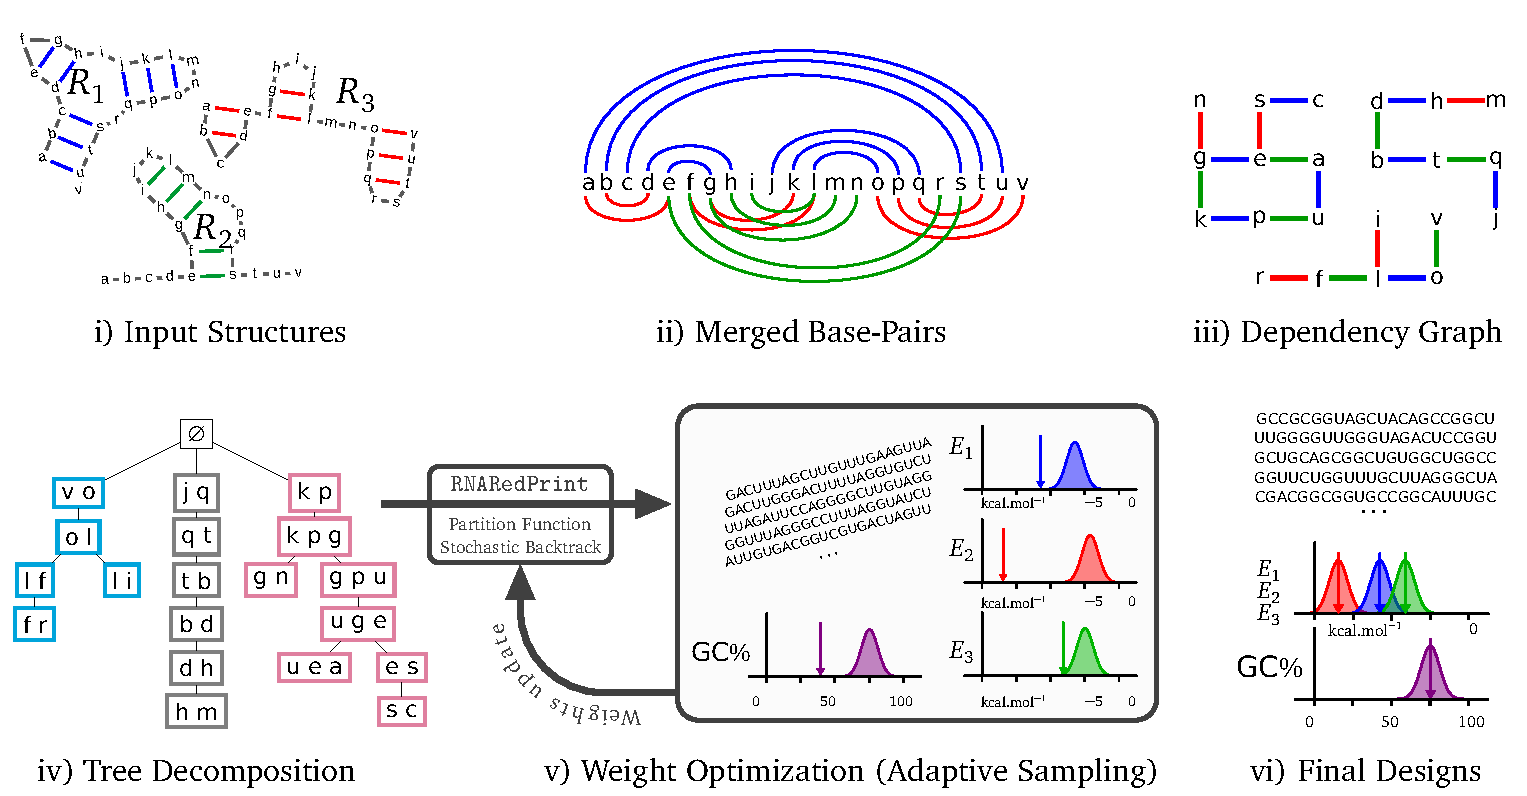
\includegraphics[width=.8\textwidth]{Figs/Workflow}
\end{center}
\caption{General outline of \ourprog{}. From a set of target secondary structures (i), base pairs are merged (ii) into a (base pair) dependency graph (iii) and transformed into a tree decomposition (iv). The tree is then used to compute the partition function, followed by a Boltzmann sampling of valid sequences (v). An adaptive scheme learns weights to achieve targeted energies and \GCb\% \revisedOne{(arrows)}, leading to the production of suitable designs (vi). \revisedOne{Note that for simplicity, we assume in this figure that only dependencies between the ends of base pairs are considered to evaluate the energies of structures. Our computations based on a more complex energy model, which considers energy contributions of base pair stacks, require additional dependencies.}
  }
\label{fig:workflow}
\end{figure*}

\revisedOne{As central contribution, we provide a systematic and flexibly extensible technique for sampling that targets multiple versatile features. For the sake of clarity, we introduce this method specialized to the sampling of RNA sequences that have specific energies for multiple structures and specific \GCb\%.}
\revised{In this way, we address the positive design of RNA sequences. Positive design is contrasted to the often
desirable negative design of RNAs, which optimizes the stability of the target structures \emph{in relation to all
other potential structures}. Remarkably, the even more complex task of negative design immediately benefits from positive
design (Additional file 1: Section~\ref{appsec:immediate-benefits-for-negative-design}), which provides an initial motivation to study the positive design problem by itself.}

\revisedOne{Figure~\ref{fig:workflow} summarizes our generic framework, which enables this targeted sequence generation based on multi-dimensional Boltzmann sampling. \emph{Algorithmically}, we originally contribute} dynamic programming (DP) algorithms, based on the concept of \Def{tree decomposition}, to compute partition functions and sample sequences from the Boltzmann distribution%
% (Subsection~\ref{sec:PF})
.
\revisedOne{Generally, tree decompositions are data structures that capture the specific dependencies of a problem instance (here, the dependencies between sequence positions induced by the target structures), such that they can guide the efficient processing by DP algorithms.}
%
\revisedOne{Building on this principle, the complexities of our algorithms depend exponentially on a specific property of the tree decomposition, called the \Def{treewidth}. Thus, it is essential for the applicability of our approach that---by appropriate design choices---we can keep this parameter low for typical instances. For} any fixed value of the treewidth, the complexity scales only linearly with the size of designed sequences and the number of targeted structures, \emph{i.e.} our algorithms are \emph{fixed-parameter tractable (FPT)}.

\revisedOne{Remarkably, we could show that it is not possible to find a better, efficient method for sampling (unless ${\sf P}={\sf NP}$), since the underlying counting problem is \#{\sf P}-hard. The practical relevance of this theoretical result is that it rules out substantially better sampling techniques. Even when using improved sampling methods, there will always remain an upper limit on the (in practice) tractable number and heterogeneity of structures, the complexity of the directly treatable energy model, and the number and complexity of additional constraints that could be considered in future sampling-based applications.} Technically, this result relies on a surprising bijection between valid sequences and independent sets of a bipartite graph, the latter being the object of recent breakthroughs in approximate counting complexity~\citep{Bulatov2013,Cai2016}.

% Subsection~\ref{sec:complexity}
%
Due to the generality of our method, we can moreover strongly limit \revisedOne{the treewidth} in practice by using state-of-the-art tree decomposition algorithms.
%Uniform sampling is handled as a special case of Boltzmann sampling, where each valid sequence receives energy zero and---consequently---computing partition functions specializes to counting.
By evaluating sequences in a specialized weighted constraint
network, we support---in principle---arbitrary \revisedOne{complex constraints and energy models},
notably subsuming the commonly
used RNA energy models%
%(Subsection~\ref{sec:energy_models})
.  Moreover, we describe an \Def{adaptive
  sampling} strategy to control the free energies of the individual
target structures and \GCb\%%
% (SubSection~\ref{sec:multiBoltzmann})
. %

We observe that
targeting realistic RNA energies in the
Turner RNA energy model
works well by performing sampling based on \revisedOne{a simplified RNA energy model, which induces much lower treewidth than the Turner model}. This result is \revisedOne{essential for the applicability of our method, since it allows to combine high efficiency (by keeping the treewidth low) with sufficient accuracy to precisely target realistic Turner energies.} 

\revisedOne{Eventually, our proof-of-concept results 
 on a comprehensive multi-target RNA design benchmark~\citep{Taneda2015} 
  suggest that our sampling strategy well supports designing biologically relevant
RNAs for multiple targets.} 

\section*{Methods}
\revisedOne{The main computational problem addressed in this work is the positive design of RNA sequences for multiple target structures; more specifically, the generation of sequences over the alphabet $\Sigma=\{\Ab,\Cb,\Gb,\Ub\}$, such that the sequences feature a given $\GCb\%$, and have prescribed energies for a set of target secondary structures.
Here, these desired sequence properties are modeled as constraints on the values of \Def{features}, which are functions of the sequence that are expressed as sums over real-valued \Def{contributions}. Each contribution depends on the nucleotides at---typically few---specific sequence positions.}

\revisedOne{To generate diverse design candidates, we randomly generate sequences from a Boltzmann distribution. The probability of a sequence then depends on its features (e.g. the energies of the target structures), and the weight of each feature (which influences its distribution). Sampling from the (multi-feature) Boltzmann distribution requires to compute corresponding partition functions, such that we can draw sequences with probabilities proportional to their Boltzmann weight. 
On this basis, we can finely calibrate the weights, to maximize the probability that sampled sequences meet the desired target values for each feature. Together with a final rejection step this results in an effective procedure for generating highly specific sequences.}


 
\subsection*{Problem statement}
\label{sec:problem-statement}

%\paragraph{Central computational problem.}
Let us consider \revised{a set of} $\numTargetStructures$ (secondary) structures $\R = \{R_1,\dots, R_{\numTargetStructures}\}$, each abstracted as a set of base pairs, and
\revisedOne{$\numFeatures\geq \numTargetStructures$} features $F_1,\dots, F_{\numFeatures}$\revisedOne{, typically
representing the energies of the structures and additional sequence properties,} associated with weights
$\pi_1,\dots,\pi_{\numFeatures}$ \revised{in $\mathbb{R}^+$}. Our goal is to sample sequences \revisedOne{$S$ (which satisfy the base pairing rules for all structures) from the Boltzmann distribution defined by} 
\begin{equation}
\label{eq:sample-distribution}
\Pr(S\mid\pi_1,\dots,\pi_{\numFeatures}) \propto \displaystyle\prod_{1\leq \ell\leq \numFeatures}\!\! \pi_\ell^{-F_\ell(S)} \end{equation}


The workhorse of our approach is the \revisedOne{fixed-parameter tractable} computation of feature-dependent partition functions over sequences, \revisedOne{namely partition functions of the form} 
%
  \begin{equation}
    \label{eq:mainproblem}
    \partfun{\pi_1,\dots,\pi_{\numFeatures}} = \sum_{S\in\Sigma^n} \prod_{1\leq \ell\leq \numFeatures} \pi_\ell^{-F_\ell(S)},
  \end{equation}
  for specific weights $\pi_1,\dots,\pi_{\numFeatures}$.

\subsection*{Expressing \GCb\%-content, sequence validity and energies as features}
Formally, we define a \Def{feature $F$} as a function on sequences, whose value is obtained by summing over an associated set of \Def{contributions}. Each contribution $f$ takes values in $\mathbb{R}\cup \{+\infty\}$, and depends on the nucleotides assigned to a restricted set of positions, \revisedOne{namely its \emph{dependencies}, denoted $\dep(f)$}, such that

$$
F(S) =\!\!\!\!\!\!\!\sum_{\substack{\text{$f$ contribution of $F$,}\\\text{ $\dep(f)=\{x_1,\ldots,x_p\}$}}}\!\!\!\!\!\! f\left(\left\{\substack{x_1\mapsto S_{x_1}\\\cdots\\x_p\mapsto S_{x_p}}\right\}\right).
$$
\revisedOne{Here, since $\dep(f)=\{x_1,\ldots,x_p\}$, $\left\{\substack{x_1\mapsto S_{x_1}\\\cdots\\x_p\mapsto
S_{x_p}}\right\}$ denotes the assignment, that assigns the respective nucleotides $S_{x_q}$ ($1\leq q\leq p$;
$p=|\dep(f)|$)} \revised{to the positions $x_q$  in $\dep(f)$}. 

The $\GCb\%$ can be simply expressed using $n$ contributions $f^{\GCb}_i$, \revisedOne{each depending only on position $i\in[1,n]$, i.e.~$\dep(f^{\GCb}_i)=\{i\}$}, such that 
$$f^{\GCb}_i(\{i\mapsto c\})=\begin{cases}-1&\text{ if }c=\Gb\text{ or }\Cb\\ 0&\text{ otherwise}.\end{cases}$$ 

\revisedOne{By summing $f^{\GCb}_i(\{i\mapsto S_i\})$ over the whole sequence ($i=1,\dots,n$), one simply counts the occurrences of $\Gb$ and $\Cb$.}

\revisedOne{
  To start with a simple example of evaluating the energy of sequences by features, let us explain how they are used to count the number of \Def{valid sequences}, \emph{i.e.} sequences inducing only base pairs in $\mathcal{B}:=\{\{\Ab,\Ub\}, \{\Gb,\Cb\}, \{\Gb,\Ub\}\}$. Consider a feature $F^{\tt BP}$ composed of  contributions $f^{\tt BP}_{i,j}$, for each base pair $(i,j)$ occurring in some structure, such that 
	$$f^{{\sf BP}}_{i,j}(\left\{\substack{i\mapsto a\\j\mapsto b}\right\})=\begin{cases}0&\text{ if }\{a,b\}\in\mathcal{B} \\+\infty&\text{ otherwise}.\end{cases}$$ 
        The value of $F^{\tt BP}$ is $0$ for any valid sequence, and $+\infty$ as soon as some non canonical base pair is created. For any associated weight $\pi_{{\sf BP}}>1$, the contribution of a valid sequence is $\pi_{{\sf BP}}^0 = 1$, and the contribution of an invalid sequence is $\pi_{{\sf BP}}^{+\infty} = 0$, so that Eq.~\ref{eq:mainproblem} (when restricted to $F^{\tt BP})$ simply counts the number of valid sequences.


Energy models for structure prediction vary considerably, yet can always be expressed as sums over contributions
associated with local structural motifs (base pairs, base pair stacks, loops, \ldots) under a certain nucleotide
assignment. Energy models can thus be captured generically by introducing, for each motif $\motif$ occurring in
a target structure, a contribution $f_{\motif}$, taking a specific value for each assignment of nucleotides to its
positions $\dep(f_{\motif})$. For instance, the contribution of a \Def{base pair stack}, consisting of two pairs $(i,j)$ and $(i+1,j-1)$, can be captured by the introduction of a function $f^{\textsf{Stack}}_{\substack{i,j}}$ such that $\dep(f^{\textsf{Stack}}_{\substack{i,j}}) = \{i,i+1,j-1,j\}$.
We refer to energy models that consider the contributions of all base pair stacks (and thus introduce the corresponding
dependencies) collectively as the \Def{stacking energy model} \revised{(briefly, \Def{stacking model})}.
}



%For the definition of energy features, we abstract an \Def{RNA (secondary) structure} $R$ of length $n$ as a set of \Def{base pairs} $(i,j)$, where
%$1\leq i<j\leq n$ and for all different $(i,j), (i',j')\in R$: $\{i,j\}\cap\{i',j'\}=\emptyset$ (``degree $\leq$ 1'')---without precluding pseudoknots.
% We call an RNA structure $R$ \Def{non-crossing}, iff it does not
% contain any two different base pairs $(i,j)$ and $(i',j')$ such that
% $i\leq i'\leq j \leq j'.$


%Moreover, in a simple \Def{base pair energy model}, the energy of a target structure $R$ is expressed as a feature associated with contributions $f^R_{ij}(\{i\mapsto x, j\mapsto y\})=\EbpSym(x,y)$ for each base pair $(i,j)$ of $R,$ such that $F^R(S)=\EbpSym(S,R)$. 


%Note that the \GCb\% as well as for the base pair energy features, the contributions depend on the nucleotides at only a small, constantly bounded, number of sequence positions (one and two positions, respectively). 

%This is important for the efficiency of our approach, which is designed to profit from contributions that each depend on only few sequence positions. 
%We emphasize that nevertheless, the same framework can capture more expressive RNA energy models like the Turner energy model~\citep{Turner2009}, since such models generally define a function $E$ that maps a pair of a sequence $S$ and a structure $R$ to a real value, the \Def{energy} $E(S,R)$. Here, our approach automatically adapts to the more complex energy functions, leading to a controlled increase of the computational complexity.

%Typically, such \Def{energy functions} are additively composed from \Def{energy contributions} of structure elements (like single base pairs or loops). It is most instructive, and in this context already practically useful, to develop our approach for the simple \Def{base pair energy model}. This model defines energy contributions $\EbpSym(x,y)$ for pairs $(x,y)\in\Sigma^2$ that specify the energy function as
%$
%\EbpSym(S,R) = \sum_{(i,j)\in R} \EbpSym(S_i,S_j)
%$
%for each sequence $S\in\Sigma^n$ and structure $R$ for length $n$.

%As the structural targets of our design, we fix the set $\R:=\{R_1, \dots, R_k\}$ of $k$ RNA structures for sequences of length $n$.
%Recall that we aim to generate random sequences that satisfy a number of constraints like the compatibility of paired bases. Moreover, we want to enforce complex properties, which we express in terms of \emph{features}. An example of such a feature is the \GCb\% (the corresponding property of a sequence is to have a specific \GCb\%). The additional properties that we are going to enforce are specific 'target' energies for the single structures $R_1, \dots, R_k$; for this purpose, each such energy is considered as a feature.

%Finally, to stress the analogy to, in the RNA context more familiar (e.g.~\citep{McCaskill1990}), Boltzmann distributions over the structure ensemble of a sequence $S$, we emphasize the equivalence
%\begin{equation}
%\label{eq:feature-energy-transformation}
%\prod_{1\leq \ell \leq k} \pi_\ell^{-F_\ell(S)} = exp(-\beta E(S)),
%\end{equation}
%where $\beta$ denotes inverse temperature and $E(S)$ is defined as linear combination of energies $E(S)=\sum_{1\leq \ell \leq k} \ln(\pi_\ell)/\beta E(S,R_\ell)$,
%where the energy $E(S,R_\ell)$ is treated as feature $F_\ell(S) = \EbpSym(S,R_\ell);$ as elaborated later, even Turner energies or pseudoknot energies can be expressed as features due to their additive nature. 

\subsection*{Dependency (hyper)graph, tree decomposition and treewidth}

%The complexity of the central problem depends fundamentally on the dependency structure that is imposed by the entire set of contributions.

%For design in the base pair energy model or the related counting problem, the dependencies are immediately derived from the set of target structures $\R$. 

%Typically, such RNA energy models consider a sequence $S$ \Def{valid} for $R$, iff $\{S_i,S_j\}\in \B$ for
%all $(i,j)\in R$, where $\B:=\left\{\{\Ab,\Ub\},\{\Gb,\Cb\},\{\Gb,\Ub\}\right\}$ describes the valid base pairs.

\revisedOne{In order to compute the partition function of Eq.~\ref{eq:mainproblem}, and thus sample in a well-defined way, one must consider dependencies induced by the complete set of contributions $$\F := \bigcup_{\ell}\{f\mid f\text{ contribution of } F_\ell\}.$$}

%
%Let us denote the \emph{dependencies of a contribution $f$} as \dep{f}.
%

\revisedOne{
In the simplest case, this set captures the requirement of canonical base pairing for each structure.
To express this, let us define the \Def{base pair dependency graph} $G_{\R}$ as the graph with nodes $\{1,\dots,n\}$
and edges $\bigcup_{\ell\in[1,\numTargetStructures]} R_\ell$. 

Since $\F$ defines potentially more complex dependencies, which can
relate more than two positions, in general its dependencies cannot be 
represented by a graph. Instead, this requires a structure known as
\Def{hypergraph}, which consists of vertices (here, the sequence
positions) connected by \Def{hyperedges}, which are arbitrary sets of
vertices. In this way, hypergraphs generalize undirected graphs where
each edge is a set of exactly two vertices.
%
The \Def{dependency (hyper)graph induced by $\F$} is then defined as the hypergraph $G_\F=(V, H)$ on sequence positions $V=\{1,\dots,n\}$
by interpreting the dependencies as hyperedges, i.e. $H =
\{\dep(f)\mid f\in \F\})$.

Let us finally define the \Def{tree decomposition} of the graph $G_\F$, a fundamental ingredient of our algorithms, which also determines their efficiency (most importantly, via its property called treewidth).
}
\begin{definition}[Tree decomposition and treewidth]
  \label{def:treedecomp}
  Let $G=(X, E)$ be a (hyper)graph with nodes in $X$ and (hyper)edges in $E$. A \Def{tree decomposition} of $G$ is
  a pair $(T,\chi)$, where $T$ is an unrooted tree/forest and, for
  each $v\in T$, $\chi(v)\subseteq X$ is a set of vertices assigned to
  the node $v\in T$, such that
\begin{enumerate}
\item each $x\in X$ occurs in at least one $\chi(v)$;
\item for all $x\in X$, $\{ v \mid x \in \chi(v) \}$ induces a connected subtree of $T$;
\item for all $e\in E$, there is a node $v\in T$, such that $e\subseteq\chi(v)$.
\end{enumerate}

\smallskip
\noindent
The \Def{treewidth} of a tree decomposition $(T,\chi)$ is defined as
$\max_{u\in T} |\chi(u)| - 1.$ 
%The \Def{treewidth} of a graph $G$ is the smallest treewidth of any tree decomposition of $G$.
\end{definition}
%
\revisedOne{Intuitively, a tree decomposition of an (hyper)graph $G$ is a tree that captures all the vertices and (hyper)edges of $G$, and properly relates dependent sub-problems to ensure consistency in a recursive computation. Figure~\ref{fig:treedec} shows an optimal tree decomposition for a pair of structures under the stacking energy model.}

\begin{figure}
{\centering 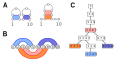
\includegraphics[width=.9\linewidth]{Figs/example-treedec-stacking}\\}
\caption{\revisedOne{Toy example of a tree decomposition associated with two target structures in the stacking energy model (where the four positions of each base pair stack depend on each other). Two target secondary structures ({\bfseries\sffamily A}) are merged into a joint hypergraph ({\bfseries\sffamily B}), whose hyperedges correspond to the quadruplets of positions involved in base pair stacks (colored). A valid tree decomposition ({\bfseries\sffamily C}) for the hypergraph ensures, among other properties, that each base pair and each base pair stack is represented in at least one of its node, so that features can be correctly evaluated. The treewidth of this tree decomposition is 3, a provably optimal value for this input hypergraph.}\label{fig:treedec}}
\end{figure}

\subsection*{Fixed-parameter tractable (FPT) algorithm}
\label{sec:FPT}

%We express our algorithms in the formalism of constraint networks, here
%specialized as RNA design network. This abstraction allows us to base our
%algorithm on cluster tree elimination (CTE)~\citet{Dechter2013}.

%The RNA design network describes how to evaluate RNA sequences and, in
%particular, partial RNA sequences, which is 

Our algorithms specialize the idea of cluster tree elimination (CTE)~\citep{Dechter2013}, which operates on constraint networks. In this correspondence, (partial) sequences specialize (partial) assignments and the constraint network would be given by variables for each sequence position, constraints due to valid base pairing, and the set of atomic feature contributions $\cal F$.


To formalize our algorithms, which iteratively merge evaluations of partial solutions, we extend the idea of atomic feature contributions, which are evaluated at sets of the form $\{x_1\mapsto v_1, \dots, x_d\mapsto v_p\}$. Let us call the latter object a \Def{partial sequence}. Such an object will help \revisedOne{to} specify partial knowledge on the sequence at some point of the algorithm. Easily, we can extend the definition of contributions $f$ to sets $\{x_1\mapsto v_1, \dots, x_p\mapsto v_p\}$, where $\{x_1\dots x_p\}$ is any super-set of $\dep(f)$ by ignoring the superfluous assignments $x\mapsto v$, where $x\not\in\dep(f)$. 

%\begin{definition}
%An \Def{RNA design network} (for sequences of length $n$) is a tuple $\network=(\X,\F)$, where
%\begin{itemize}
%\item $\X$ is the set of sequence positions $1,\dots,n$
%\item $\F$ is a set of \Def{contributions} $f:\Sigma^n\to\real$
%\end{itemize}
%\end{definition}
%
%Notably the term `network' refers to the implied graph structure, namely the dependency graph.

%\newcommand{\weighttransform}[2]{{#1}_{||{#2}}}

Moreover, to ensure a uniform algorithmic treatment of contributions, it is convenient to encode the weight $\pi$ of each feature in its contributions. This transformation works by multiplying all contributions with $\ln(\pi)$, where $\pi$ is the weight of the corresponding feature, since then
$exp(-\ln(\pi)f(S))=\pi^{-f(S)}.$

%For this purpose, we define the \Def{transformed contribution} 
%$\weighttransform{f}{\pi}(S) := \ln(\pi)f(S),$
%such that $exp(-\weighttransform{f}{\pi}(S))=\pi^{-f(S)}.$ 
%
Let us now specify the concrete set $\F$ of contributions that we use
for the design in the stacking energy model targeting \GCb\% and structures $\R$ with weights $\pi_0,\dots,\pi_k$. The set $\F$ thus consists of
\begin{itemize}
\item the transformed contributions $\ln(\pi_0)f^{\GCb}_i$ for the ~$\GCb\%$ feature ($i=1,\dots,n$);
\item the transformed contributions $\ln(\pi_\ell)f^{{\textsf{Stack}}}_{ij}$ for each structure $R_\ell\in\R$ and $(i,j)\in R_\ell.$
\end{itemize}
%
By these definitions, the set $\F$ encodes the partition function $\partfun{\pi_0,\dots,\pi_k}$ of Eq.~(\ref{eq:mainproblem}).
%Subsequently, we show how to efficiently compute this partition function based on the 
%corresponding dependency graph and its tree decomposition.


\subsubsection*{Partition function and stochastic backtracking}\label{sec:PF}

We compute the partition function (as specified by $\F$) by dynamic programming based
on a tree decomposition of $G_{\F}$, the dependency graph associated with $\F$.
Note, that analogous algorithms could be easily derived to count valid sequences, or list sequences having minimum free
energy.
%This yields fixed parameter tractable (FPT) algorithms, based on the treewidth.

%\begin{figure}[t]
%{\centering\scalebox{11}{\fbox{$\phantom{5689}$}}\\}
%
%  \caption{Figure illustrating RNA network to hypergraph to tree decomposition}
%\end{figure}

Our algorithms are formulated to process a \Def{cluster tree} of $\F$, which is a tuple $(T,\chi,\phi)$, where
$(T,\chi)$ is a tree decomposition of $G_\F$, and $\phi(v)$ represents
a set of functions $f$, each uniquely assigned to a node $v\in T$;
$\dep(f)\subseteq\chi(v)$ and $\phi(v)\cap \phi(v')=\varnothing$ for
all $v\neq v'$. 

Two further notions are essential for our algorithms: for two nodes $v$ and $u$ of the cluster tree, define
their \Def{separator} as $\separator{u}{v} := \chi(u)\cap\chi(v)$;
moreover, we define the \Def{difference positions} from $u$ to an
adjacent $v$ by $\difference{u}{v}:=\chi(v) - \separator{u}{v}$.

Since our algorithms iterate over specific sets of sequence positions, we moreover define
the \Def{set $\partseqs(\Y)$ of all partial sequences determining the positions of $\Y\subseteq\{1,\dots,n\}$} in all combinations of nucleotides $\{\Ab,\Cb,\Gb,\Ub\}$,
i.e.~for $\Y=\{y_1,\dots,y_{q}\}$,
\begin{align*}
\partseqs(\Y) = \{ & \{ y_i\mapsto v_i \mid i=1,\dots,q \} \\& | (v_1,\dots,v_{q}) \in \{\Ab,\Cb,\Gb,\Ub\}^{q} \}.
\end{align*}
%
We assume the following properties of the given cluster tree (reflecting $\F$):
\begin{itemize}
\item
$T$ is
connected and contains a dedicated node $r$, with
$\chi(r)=\varnothing$ and $\phi(r)=\varnothing$. If such a root does not exist, it can be added to the tree decomposition and connected to one node in each connected component of $T$;
\item
all edges in the tree decomposition are oriented towards this root;
\item
all sets $\difference{u}{v}$ are singleton: for any given
cluster tree, an equivalent (in term of treewidth) cluster tree can
always be obtained by inserting at most $\Theta(|\X|)$ additional
clusters.
\end{itemize}

Algorithm~\ref{alg:pf} computes the partition function by passing
messages along the directed edges $u\to v$ (which point from 
child $u$ to its parent $v$). Each message $m$ has the form of a contribution, i.e. it takes a partial sequence, depends
on the positions $\dep(m)\subseteq \X$, and yields a partition function
in $\real$. The message from $u$ to $v$ represents the
partition functions of the subtree of $u$ for all possible partial
sequences in $\partseqs(\separator{u}{v})$. Induction over $T$ lets us show
the correctness of the algorithm
(Additional file~1: Section~\ref{appsec:correctness}).  After running
Alg.~\ref{alg:pf}, multiplying the 0-ary messages sent to the root $r$
yields the total partition function (i.e.~due to proper encoding the partition function of our design problem) through
\begin{math}
  \prod_{(u\to{}r)\in T} \evalfor{\Message{u}{r}}{\varnothing}.
\end{math}


\begin{algorithm}[t]
  \KwData{Cluster tree $(T,\chi,\phi)$} \KwResult{Messages
    $\Message{u}{v}$ for all $(u\to{}v)\in T$; i.e.~partition
    functions of the subtrees of all $v$ for all possible partial
    sequences determining exactly the positions $\separator{u}{v}$.}
  \For{$u\to{}v\in T$ in postorder}{
    \For{$\val\in\partseqs(\separator{u}{v})$}{
      $x\gets 0$\;
      \For{$\val'\in\partseqs(\difference{u}{v})$}{
        $p \gets$ product( $exp(-\evalfor{f}{\substitute{\val}{\val'}})$ for $f\in \phi(u)$ )\\
        ${}\quad\qquad \cdot\ $product( $\evalfor{\Message{u'}{u}}{\substitute{\val}{\val'}}$ for $(u'\to{}u)\in T$ )\;
        $x \gets x + p$\;
      }
      $\evalfor{\Message{u}{v}}{\val} \gets x$\;
    }
    \Return {$m$}\;
  }
  \caption{FPT computation of the partition function using dynamic
    programming, i.e.~cluster tree elimination (CTE). The postorder traversal guarantees that
    when processing edge $u\to{}v$, all messages
    $\Message{u'}{u}$, corresponding to DP matrices, have been computed before. }\label{alg:pf}
\end{algorithm}

The partition functions can then direct a stochastic backtracking procedure to sample sequences from the Boltzmann distribution (according to $\F$).
%
For an expanded cluster tree, after the messages $\Message{u}{v}$ for
the edges in the tree decomposition are generated by Algorithm \ref{alg:pf},
one can repeatedly call Algorithm~\ref{alg:sampling}, each time
randomly drawing another sequence from the Boltzmann distribution.

\subsection*{Complexity considerations}\label{sec:complexity}

%The complexity of the proposed sampling algorithm depends on the treewidth of the dependency graph $G_\F$.
% The treewidth $w$ of a cluster tree $(T,\chi,\phi)$, $T=(V,E)$, is $\max_{v\in V} |\chi(v)| - 1$, i.e.~the maximum number of positions in any of its clusters minus 1.
Let $s$ denote the maximum size of any separator set $\separator{u}{v}$ and $D$ denote the maximum size of
$\difference{u}{v}$ over $(u,v)\in E$.  In the absence
of specific optimizations, running Alg.~\ref{alg:pf} requires
$\mathcal{O}((|\F|+|V|)\cdot 4^{w+1})$ time and
$\mathcal{O}(|V|\cdot4^s)$ space; Alg.~\ref{alg:sampling} would
require $\mathcal{O}((|\F|+|V|)\cdot 4^D)$ per sample on arbitrary
tree decompositions
(Additional file 1: Section~\ref{appsec:algcomplexity}). W.l.o.g.\ we assume that
$D=1$; note that tree decompositions can generally be transformed,
such that $\difference{u}{v}\leq 1$.
%
Moreover, the size of $\F$ is linearly bounded: for $k$
input structures for sequences of length $n$, the energy function is
expressed by $\mathcal{O}(n\,k)$ functions. Finally, the number of cluster
tree nodes is in $O(n)$, such that $|\F|+|V| \in \mathcal{O}(n\,k)$.

% \begin{algorithm}
%  \KwData{Node $u$, partial sequence $\val\in\partseqs(\separator{u}{v})$;\newline
%  Cluster tree $(T,\chi,\phi)$ and partition functions $\Message{u'}{v'}[\val']$, $\forall (u'\to{}v')\in T$ and $\val'\in\partseqs(\separator{u'}{v'})$.}
%  \KwResult{Boltzmann-distributed random partial sequence for the subtree rooted at $u$, specializing a partial sequence $\val$.}
%  \Fn{\Sample$(u,\val)$}{
%    $r \gets \Random(\evalfor{\Message{u}{v}}{\val})$\;
%    \For{$\val'\in\partseqs(\difference{u}{v})$}{

%      $p \gets$ product( $exp(-\evalfor{f}{\substitute{\val}{\val'}})$ for $f\in \phi(u)$ )\\
%      ${}\quad\qquad \cdot\ $product( $\evalfor{\Message{u'}{u}}{\substitute{\val}{\val'}}$ for $(u'\to{}u)\in T$ )\;
%   	  $r \gets r - p$\;
%   	  \If{$r<0$}{
%   	    $\val_{\rm res} \gets \substitute{\val}{\val'}$\;
%   	  \For{$(u'\to{}u)\in T$}{
%   	      $\val_{\rm res} \gets \substitute{\val_{\rm res}}{\Sample(u',\substitute{\val}{\val'})}$\;
%      }
%   	  \Return {$\val_{\rm res}$}
%   	  \;}
%  }
%  }
%  \caption{Stochastic backtrack algorithm for partial sequences in the Boltzmann distribution.}\label{alg:sampling}
% \end{algorithm}

\begin{algorithm}
 \KwData{Cluster tree $(T,\chi,\phi)$ and partition functions $\Message{u'}{v'}$ for all $(u'\to{}v')\in T$.}
 \KwResult{One random sequence $\val$ sampled from the Boltzmann distribution}
 $\val$ \gets $\varnothing$\;
 \For{$u\to{}v\in T$ in preorder}{
   $r \gets \text{uniform random number between $0$ and $\evalfor{\Message{u}{v}}{\val}$}$\;
   \For{$\val'\in\partseqs(\difference{u}{v})$}{

     $p \gets$ product( $exp(-\evalfor{f}{\substitute{\val}{\val'}})$ for $f\in \phi(u)$ )\\
     ${}\quad\qquad \cdot\ $product( $\evalfor{\Message{u'}{u}}{\substitute{\val}{\val'}}$ for $(u'\to{}u)\in T$ )\;
     $r \gets r - p$\;
     \If{$r<0$}{
       $\val \gets \substitute{\val}{\val'}$\;
     }
   }
 }
 \Return {$\val$}\;

 \caption{Stochastic backtrack algorithm for partial sequences in the
   Boltzmann distribution. Processing the edges $u\to{}v\in T$ in
   preorder ensures that $\val$ invariantly determines all positions
   of $v$ outside the subtree of $u$.}\label{alg:sampling}
\end{algorithm}


%For example, for design to a single non-crossing target in the nearest neighbor energy model, the complexity of Algs.~\ref{alg:pf} and \ref{alg:sampling} degrades to linear time (as reported for IncaRNAtion), since there are only $O(n)$ many functions and nodes (in the sequence length $n$). Moreover, the dependencies are tree-like owing to the tree-like non-crossing structure; this implies a constantly bounded maximum treewidth.


\begin{theorem}[Complexities]\label{th:complexities}
  \revised{Given are sequence length $n$, $k$ target structures, and tree\-width $w$.
  % and a base pair dependency graph having $c$ connected components%
  $t$ sequences
  are generated from the Boltzmann distribution  in
  $O( n\, k \, 4^{w+1} + t\, n\, k )$ time.}
  %$O( n\, k \min(2^{w+c+1},4^{w+1}) + t\, n\, k )$ time.
  %$\mathcal{O}( 2^d\, n\, k  + t\, n\, k )$ time, where $d:=\min(w+c+1,2(w+1))$.
\end{theorem}

By this theorem, the complexity is polynomial for fixed value of $w$, and Boltzmann sampling in our setting is thus fixed parameter tractable (FPT) in the treewidth.
%
The complexity of the precomputation can be further improved to
$\mathcal{O}(n\,k\,2^{w+1}\,2^{c})$, where $c$ ($c\le w+1$) is the maximum number of connected components represented in a node of the tree decomposition (Additional file~1: Section~\ref{appsec:improvedComplexity}).


Note that in this complexity analysis, we do not include time and space for computing the
tree decomposition itself, since we observed that the computation time
of tree decomposition (\Software{GreedyFillIn}, implemented in
\Software{LibTW}~by \citet{Dijk2006}) for multi-target sampling is
negligible compared to Alg.~\ref{alg:pf}
(Additional file~1: Sections~\ref{appsec:treedecomp} and
\ref{appsec:dependency-cliques}).

\subsection*{Design within expressive energy models}\label{sec:energy_models}

% \paragraph{Nearest-neighbor model.}
% Let us now consider a simplified version of the nearest-neighbor model, where the free energy contribution  $\Ehp{x,y,s}$ of a hairpin only depends on the closing base pair $(x,y)$, and the contribution $\Eint{x,y,x',y',s}$ of an interior loop depends on its opening/closing bases pairs $(x,y)/(x',y)$, and its length $s$. Moreover, the energy of a multi loops with $s$ inner base pairs and $t$ unpaired base pairs is approximated as $a+b\,s+c\,t$, where $a,b,c$ are predefined constants.

% Again, the energy is expressed by adding functions to $F$ for each $R_\ell$ and base pair $(i,j)\in R_\ell$:
% \begin{itemize}
%   \item if $(i,j)$ closes a hairpin in $R_\ell$, add $f$, s.t.~$\evalfor{f}{\val_S}=\Ehp{S_i,S_j,j-i}$
%   \item if $(i,j)$ closes an interior loop, bulge or stack with inner base pair $(i_1,j_1)$ in $R_\ell$, add $f$, s.t.~$\evalfor{f}{\val_S}=\Ehp{S_i,S_j,S_k,S_l,i_1-i+j_1-j}$
%   \item if $(i,j)$ closes a multiloop add $f$, s.t.~$\evalfor{f}{\val_S}=a$.
%   \item if $(i,j)$ is inner base pair of a multiloop of $R_\ell$ add $f$, s.t.~$\evalfor{f}{\val_S}=b$.
% \end{itemize}
% Finally add for each $R_\ell$ and unpaired base $i$ in a multi loop of $R_\ell$, the function $f$, $\evalfor{f}{\val_S}=c$.

In order to capture realistic energy models like the Turner model or pseudoknot models like {\tt
HotKnots}~\citep{Ren2005}, our sampling strategy can be extended in two ways: 1) either by directly sampling based on
more expressive energy models \revisedOne{or 2) by sampling in a simple energy model which} can be used to approximate
sampling in more complex models.  In practice, complex energy models \revisedOne{have} a strong influence on the
treewidth (of optimal tree decompositions) of the dependency graph and \revisedOne{thus on} the computational complexity
of our approach. Therefore, it is interesting to consider---in addition to the \revised{stacking energy model}---other
stripped-down variants of the nearest neighbor model, which could offer a compromise between \revised{low-complexity (as due to
the stacking energy model) and the high-accuracy of the Turner model.}


\paragraph{Exact energy models.}
A first model, which is particularly promising, is the
\Def{stacking energy model}. This model only assigns energy
contributions $\Delta G(x_i,x_j,x_{i+1},x_{j-1})$ to stacks consisting of two nested base pairs $(i,j)$ and $(i+1,j-1)$. Within our framework, this energy model is captured by contributions $f_S(\{x_i\mapsto s_i, x_{i+1}\mapsto s_{i+1}, x_{j-1}\mapsto s_{j-1}, x_{j}\mapsto s_{j}\}):=\Delta G(x_i,x_j,x_{i+1},x_{j-1})$ associated with stacks occurring in at least one of the input structures.

Complex \Def{loop-based} energy models---e.g.~the Turner model which, among others, includes energy terms for special loops and dangling
ends---can also be encoded exactly as instances of our general framework. Namely, each loop $L$ involving positions $x_1$,\ldots,$x_p$ will be modeled by a contribution $f_L(\{x_1\mapsto s_1,\ldots, x_p\mapsto s_p\}):=\Delta G(s_1,\ldots,s_p)$, where $\Delta G(s_1,\ldots,s_p)$ is the energy assigned to the loop in the energy model for a given nucleotide content $s_1,\ldots,s_p$. Note that the maximum arity of contributions constitutes a lower bound on the treewidth, which may impact the practical complexity of our algorithms. For instance, loop contributions in the Turner 2004 model~\citep{Turner2009} may depend on up to
nine bases for interior loops, with a total of 5 unpaired bases (``2x3'' interior loops)--- although all other energy contributions, including dangling ends, only depend on at most four nucleotides.


%The arity of the introduced functions influences the
%treewidth of the dependency graph.
%Thus, it is noteworthy that the base pair energy model
%requires only binary functions; the stacking model, only quarternary
%dependencies. This arity is increased in a few cases by the commonly
%used Turner 2004 model~\citep{Turner2009} for encoding tabulated
%special hairpin and interior loop contributions, which depend on up to
%nine bases for the interior loops with a total of 5 unpaired bases
%(``2x3'' interior loops)---all other energy contributions (like
%dangling ends) still depend on at most four bases of the sequence.


\paragraph{Approximating Turner Energy using Simpler Energy Models.}
To capture the realistic Turner model $\EnergyTurner$ more efficiently, we exploit the tight correlation between
$\EnergyTurner$ and the fitted stacking model $\EnergyStacking$
(Additional file~1: Section~\ref{appsec:modelparameters}). More precisely, we observed a
structure-specific affine dependency between the Turner and stacking
energy models, so that
$\EnergyTurner(S;R) \approx \gamma\cdot \EnergyStacking(S;R) + \delta$
for any structure $R$ and sequence $S$. We inferred the
$(\gamma,\delta)$ parameters from a set of sequences generated with
homogeneous weights $w=e^{\beta}$, tuning only \GCb\% to a
predetermined value.  Finally, we adjusted the targeted energies
within our stacking model to
$\EnergyStacking^{\star} = (\EnergyTurner^{\star}- \delta)/\gamma$ in
order to reach, on average, the targeted energy
$\EnergyTurner^{\star}$ in the Turner model.


\subsection*{Extension to multidimensional Boltzmann sampling}\label{sec:multiBoltzmann}
The flexibility of our framework allows to support the advanced sampling technique called "multidimensional Boltzmann sampling"~\citep{Bodini2010}, which allows to enforce (probabilistically)  additional, complex properties of the samples through an additional rejection.
This technique was previously used to control \GCb\%~\citep{Waldispuehl2011,Reinharz2013} and di-nucleotide
content~\citep{Zhang2013} of sampled RNA sequences. Here, in addition to controlling \GCb\% (our feature $F_0$) we use
it to target the free energies $(\TargetE_1,\ldots,\TargetE_{\numTargetStructures})$ of the individual target structures (features
$F_1,\dots,F_{\numFeatures}$).

For the multidimensional Boltzmann sampling, we require the already established ability to \Def{sample from a weighted distribution} over the set of valid sequences, where the probability of a sequence $S$ is
$$\mathbb{P}(S\mid \pmb{\pi}) = \frac{\prod_{\ell=0}^{k} \pi_i^{-F_i(S)}}{\partfun{\pmb{\pi}}},$$
where $\pmb{\pi}:=(\pi_0\cdots\pi_k)$ is the vector of the positive real-valued \Def{weights}, and $\partfun{\pmb{\pi}}$ is the weighted partition function.

%Such a distribution can be induced by a simple modification of the functions described in Sec.~\ref{sec:energy_models}, where any energy function $E(\val)$ for a structure $\ell$ is replaced by $E'(\val):= \ln(\pi_\ell)\, E(\val)/\beta.$ 
%Due to the construction of $\F$,
%the probability of a sequence $S$ is thus proportional to
%$\prod_{\ell=0}^{k} \pi_i^{-F_i(S)} = \prod_{f\in\F} f(S).$

One then needs to \Def{learn a weights vector} $\pmb{\pi}$ such that, on average, the targeted energies are achieved by a random sequences in the weighted distribution. In other words,  $\mathbb{E}(F_\ell(S)\mid \pmb{\pi})=\TargetE_\ell$,  $\forall\ell\in[1,k]$ and, analogously, the expectation of $F_0(S)$ is the targeted GC content.
The expected value of $F_\ell$ is always decreasing for increasing weights $\pi_\ell$ (see Additional file~1: Section~\ref{appsec:weight_derivatives}).
More generally, computing a suitable parameter vector $\pmb{\pi}$ can be restated as a convex optimization problem, and be efficiently solved using a wide array of methods~\citep{Denise2010,Bendkowski2017}.

In practice, we use a simple heuristics which starts from an initial weight vector $\pmb{\pi}^{[0]}:=(e^\beta,\dots,e^\beta)$ for $\beta=1/(RT)$, T=$37^\circ$, and gas constant $R$. Then, at each iteration, it generates samples $\mathcal{S}$ of sequences. The expected value of an energy $F_\ell$ is estimated as $\hat\mu_\ell(\mathcal{S}) = \sum_{S\in\mathcal{S}}F_\ell(S)/|\mathcal{S}|$, and the weights are updated at the $t$-th iteration by %  $\pi_\ell^{[t+1]} = \pi_\ell^{[t]}\cdot\TargetE_\ell/\hat\mu_\ell(\mathcal{S})$.
$\pi_\ell^{[t+1]} = \pi_\ell^{[t]}\cdot \gamma^{\hat\mu_\ell(\mathcal{S})-\TargetE_\ell}$. In practice, the constant $\gamma>1$ is chosen empirically  ($\gamma=1.2$) to achieve effective optimization.
While heuristic in nature, this basic iteration was elected in our initial version of \ourprog{} because of its good empirical behavior.

A further \Def{rejection step} is applied to retain only those sequences whose energy for each structure $R_\ell$ belongs to $[\TargetE_\ell\cdot(1-\varepsilon),\TargetE_\ell\cdot(1+\varepsilon)]$, for $\varepsilon\ge 0$ some predefined \Def{tolerance}. The rejection approach is justified by the following considerations:
i) \emph{Enacting an exact control over the energies would  be technically hard and costly.} Indeed, controlling the energies through dynamic programming would require explicit convolution products, generalizing~\citep{Cupal1996}, inducing additional $\Theta(n^{2k})$ time and $\Theta(n^k)$ space overheads;
ii) \emph{Induced distributions are typically concentrated.} Intuitively, unless sequences are fully constrained individual energy terms are independent enough so that their sum is concentrated around its mean -- the targeted energy (cf.{} Fig.~\ref{fig:energydist-pk}).
%Indeed, as shown in Fig.~\ref{fig:shifting_mean}, empirical joint distributions in the energies have good fits towards Normal multidimensional distributions with linear (co-)variances.
For base pair-based energy models and special base pair dependency graphs
(paths, cycles\ldots) this property rigorously follows from analytic
combinatorics, see \citep{Bender1983} and
\citep{Drmota1997}. In such cases, the expected number of
rejections before reaching the targeted energies remains constant when
$\varepsilon\ge 1/\sqrt{n}$, and $\Theta(n^{k/2})$ when
$\varepsilon=0$. 
%The \GCb\% of designs can also be controlled,
%jointly and in a similar way, as done in
%\Software{IncaRNAtion}~\citep{Reinharz2013}.

\subsection*{\#{\sf P}-hardness of counting valid designs}\label{sec:counting}
%%% reformulate later
%We define the following notations: $\real^\infty:=\real\cup\{\infty\}$, $[i,j]:=\{i,\ldots,j\},$ \ldots
\revisedOne{While efficient, both in practice and in theory for graphs of bounded treewidth, our algorithms remain exponential in the worst case scenario, since the treewidth of a dependency graph can then become arbitrarily large. This exponential complexity in the worst case appears to be intrinsic. Indeed, we show that a specialization of our core problem, namely the enumeration of designs that respect canonical base pairing rules ($\Ab \leftrightarrow \Ub$, $\Gb \leftrightarrow \Cb$, $\Gb \leftrightarrow \Ub$) is $\#{\sf P}$-hard, even when the dependency graph is bipartite and connected. The existence of a polynomial time algorithm for computing the partition function of Equation \eqref{eq:mainproblem} is thus unlikely, as it would imply that  ${\sf\# P}={\sf FP}$ and, in turn, that ${\sf P}={\sf NP}$.}

%Our contributed algorithms, while 
%Finally, we turn to the complexity of $\NumDesign(G)$, the problem of
%computing the number of valid sequences for a given compatibility
%graph $G=(V,E)$. Note that this problem corresponds to the partition
%function problem with weights $\pi_\ell=1$ for each target structure, so that each valid structure contributes $1$ to the partition
%function; each invalid structure, 0.
%
%As previously noted~\citep{Flamm2001}, a set of target
%structures admits a valid design iff its compatibility graph is
%bipartite, which can be tested in linear time.  Moreover, without
%$\{\Gb, \Ub\}$ base pairs, the design of any connected component $C$
%of $G$ would be entirely determined by the assignment of a single of
%its nucleotides. The number of valid designs is thus simply
%$4^{\#{\rm CC}(G)}$, where $\#{\rm CC}(G)$ is the \Def{number of
%  connected components}.
%The problem becomes much harder when $\{\Gb, \Ub\}$ base pairs are allowed, and we show that valid designs for a set of structures cannot be counted in polynomial time, unless ${\sf\# P}={\sf FP}$. This equality would, in particular, imply the classic ${\sf P}={\sf NP}$.

To establish that claim, we consider a dependency graph $G=(V_1\cup V_2, E)$ that is connected and bipartite ($E \cap (V_1\times V_2) = E$). Note that, assigning a nucleotide to a position $u\in V$ constrains the parity ($\{\Ab,\Gb\}$ or $\{\Cb,\Ub\}$) of all positions in the connected component of $u$. For this reason, we restrict our attention to the counting of valid designs \emph{up to trivial  symmetry} $(\Ab\leftrightarrow \Cb/\Gb\leftrightarrow \Ub)$, by constraining the positions in $V_{1}$ to $\Ab$ and $\Gb$. Let $\Design{G}$ denote the subset of all designs for $G$ under this constraint, noting that $\NumDesign(G) = 2\cdot|\Design{G}|$.

Finally, let $\IS{G}$ denote the set of all independent sets in the connected graph $G$; recall that an \Def{independent set} of $G=(V,E)$ is a subset $V'\subseteq V$ of nodes that are not connected by any edge in $E$. 

\begin{proposition}\label{prop:bijection}
  $|\Design{G}| = |\IS{G}|$.
\end{proposition}
%
\begin{proof}
  Consider the mapping\\\hspace*{2em}$\Psi: \Design{G} \to \IS{G}, f \mapsto \left\{v\in V\mid f(v)\in\{\Ab,\Cb\}\right\}.$\\
We show that $\Psi$ is bijective:%
\begin{itemize}
\item $\Psi$ is injective, i.e. $\Psi(f)\neq\Psi(f')$ for all $f\neq f'$.
If $f\neq f'$, then there exists a node $v\in V$ such that $f(v)\neq f'(v)$.
We discuss only the case $v\in V_1$, where we restricted the nucleotides to $\Ab$ and $\Gb$. Then, $\{f(v),f'(v)\}$ must equal $\{\Ab,\Gb\}$, such that either $v\in\Psi(f)$ or $v\in\Psi(f')$.
%
\item $\Psi$ is surjective, i.e. there is a preimage for each element $I\in \IS{G}$. Define $f\in\Design{G}$ as\begin{displaymath}
f(v) = \left\{\begin{array}{ll} % @{\qquad}ll
\Ab{} & \text{if $v\in V_1$ and $v\in I$} \\ %&
\Cb{} & \text{if $v\in V_2$ and $v\in I$} \\
\Gb{} & \text{if $v\in V_1$ and $v\not\in I$} \\ %&
\Ub{} & \text{if $v\in V_2$ and $v\not\in I$}
\end{array}\right.
\end{displaymath}
One easily verifies that $\Psi(f) = I$.
%
%for any $(v_1,v_2)\in V_1\times V_2$ by
%\begin{align*}
%f(v_1) &= \begin{cases} \Ab & \text{if }v_1\in S\\ \Gb & \text{if }v_1\notin S\end{cases} &
%\text{\quad and\quad}&&
% f(v_2) &= \begin{cases} \Cb & \text{if }v_2\in S\\ \Ub & \text{if }v_2\notin S.\end{cases}
%\end{align*}
%
It remains to show that $f$ is a valid design for $G$, i.e. for each $(v, v') \in E$, $\{f(v),f(v')\}\in \B$; please recall that we defined $\B$ as the set of all valid nucleotide pairs.
Assume there is an edge $(v_1,v_2)\in E$, violating $\{f(v_1),f(v_2)\} \in \B$. Since $G$ is bipartite,
$v_1\in V_1$ and $v_2\in V_2$, such that $f(v_1)\in\{\Ab,\Gb\}$ and $f(v_2)\in\{\Cb,\Ub\}$. This implies that among all possible $\{f(v_1), f(v_2)\}$ only $\{\Ab,\Cb\}$ is not in $\B$, which in turn requires $v_1\in I$ and $v_2\in I$. Therefore, since $I$ is an independent set, the edge $(v_1,v_2)\in E$ cannot exist. \QEDA
\end{itemize}
\end{proof}

Counting independent sets in bipartite graphs ($\#{\sf BIS}$) is a well-studied problem, shown to be \#{\sf P}-hard~\citep{Ge2012} even on connected graphs. Now assume the existence of an efficient (polynomial-time) algorithm $\mathcal{A}$ for computing $|\NumDesign(G)|$ on connected (bipartite) graphs. Then, running $\mathcal{A}$ and returning $|\NumDesign(G)|/2$ constitutes an efficient algorithm for $\#{\sf BIS}$ on connected graphs.
%However, $\#{\sf BIS}$ is also \#{\sf P}-hard on connected graphs, as the number of independent sets for a disconnected graph $G$ can be efficiently computed by $|\IS{G}|=\prod_{cc\in CC(G)} |\IS{cc}|$. 
In other words, any efficient algorithm for \NumDesign implies an efficient algorithm for $\#{\sf BIS}$, thus our conclusion that \NumDesign is $\#{\sf P}$-hard. 

\revisedOne{Proposition~\ref{prop:bijection} also strongly impacts the complexity of computing the partition function. Indeed it implies that, among the $4^k$ possible assignments of nucleotides to $k$ connected positions (in the base-pair dependency graph), at most $2^k$ are compatible with base pairing rules. One can thus sharply reduce the complexity of Algorithm~\ref{alg:pf} by restricting the precomputations to compatible assignments.

For a discussion on the implications of our hardness results beyond exact counting see Additional file~1: Section~\ref{appsec:approximate-counting}.
}

% \begin{proof}

%   Given any algorithm $\mathcal{A}$ that solves \NumDesign over strongly-connected graphs $G$, one can  construct an algorithm $\mathcal{A}'$ that solves $\#{\sf BIS}$:
%   \begin{enumerate}
%     \item[1)] calculate $\NumDesign(G)$ by calling $\mathcal{A}$
%     \item[2)] return\\$\NumDesign(G)/2=|\Design{G}| = |\IS{G}|$.
%   \end{enumerate}
%     Obviously, if $\mathcal{A}$ is a polynomial-time algorithm, so is $\mathcal{A'}$.
%   This implies that $\NumDesign$  is at least as hard as $\#{\sf BIS}$, thus does not admit a polynomial time exact algorithm unless $\#{\sf P}={\sf FP}$.
% \end{proof}




\section*{Results}\label{sec:results}

We implemented the core algorithms in \texttt{C++}, resulting in the tool
\ourprog{}, available at: 
%
{\url{https://github.com/yannponty/RNARedPrint}}.%

\noindent
\ourprog{}  takes a set of target structures, as well as
weights for each energy feature and \GCb\%, and generates a sample set of sequences compatible with the structures in the corresponding
Boltzmann distribution\revised{; it currently supports the stacking energy model and the base pair energy model
(Additional file~1: Section~\ref{appsec:modelparameters}).} 

Moreover, we provide two {\tt Python} wrapper scripts. 
The first script targets prescribed energies using multi-dimensional Boltzmann sampling.
For a given set of secondary structures, together with prescribed target energies
and target \GCb\%, this script generates a series of sequences that satisfy the target values for the energy and
\GCb\% features within configurable tolerances.
Notably, these target energies are actual free energies in the realistic
Turner energy model, and are targeted by efficiently sampling in the
stacking energy model, and filtering sequences based on the {\tt RNAeval} tool from the Vienna package~\cite{Lorenz2011}. The second script generates high quality seed sequences suitable for negative RNA design. The details of this approach are described in the subsections below.

\subsection*{Practical efficacy of Boltzmann sampling for sequences}

\begin{figure}
	\includegraphics[width=0.8\textwidth]{Figs/Plots/doublestem_weight1-500_mean}
	\caption{\revisedOne{Comparison of free energy and Boltzmann probability for 10~000 uniform ($\pi=1$; blue dots) and Boltzmann distributed ($\pi=500$; green dots) sequences, targeting a simple structure consisting of two adjacent helices.}}
        \label{fig:BoltzmannBenefits}
\end{figure}

\revisedOne{First, we show how seed sequences can be generated in a Boltzmann distribution, leading to designs that are substantially more stable that those generated uniformly. As can be seen in Figure~\ref{fig:BoltzmannBenefits} and Additional file~1: Section~\ref{appsec:immediate-benefits-for-negative-design}, sequences generated in the Boltzmann distribution not only reach lower free-energies than those generated in a uniform setting, but also achieve better Boltzmann probabilities. While the former is expected since the Boltzmann distribution explicitly favors low-energy candidates, the latter is somewhat surprising, since the Boltzmann probability of a target structure could, in principle, decrease under Boltzmann sampling due to the partition function growing faster than the Boltzmann factor. The empirical superiority of Boltzmann sampling appears robust to the target structure length and topology, as demonstrated by prior work~\cite{Reinharz2013}.}
	
\begin{figure}
	  \begin{minipage}{.35\textwidth}\centering 
{\sffamily {\bfseries A} -- 
	Stacking model}\\
	\resizebox{\textwidth}{!}{
		\begin{tabular}{c|c@{\hspace{.5em}}c@{\hspace{.5em}}c@{\hspace{.5em}}c@{\hspace{.5em}}c@{\hspace{.5em}}c}
		$\Delta G$ 	& \Ab\Ub & \Cb\Gb & \Gb\Cb & \Gb\Ub & \Ub\Ab & \Ub\Gb \\[.4em]\hline
			\Ab\Ub &
			-0.18&
			-1.13&
			-1.09&
			-0.38&
			-0.26&
			-0.62
			\\[.4em]
			\Cb\Gb&
			-1.11&
			-2.23&
			-1.89&
			-1.22&
			-1.10&
			-1.44
			\\[.4em]
			\Gb\Ub&
			-0.55&
			-1.26&
			-1.58&
			-0.72&
			-0.50&
			-0.69
			\\
	\end{tabular}}\\[3em]
{\sffamily {\bfseries C} -- Treewidths}\\
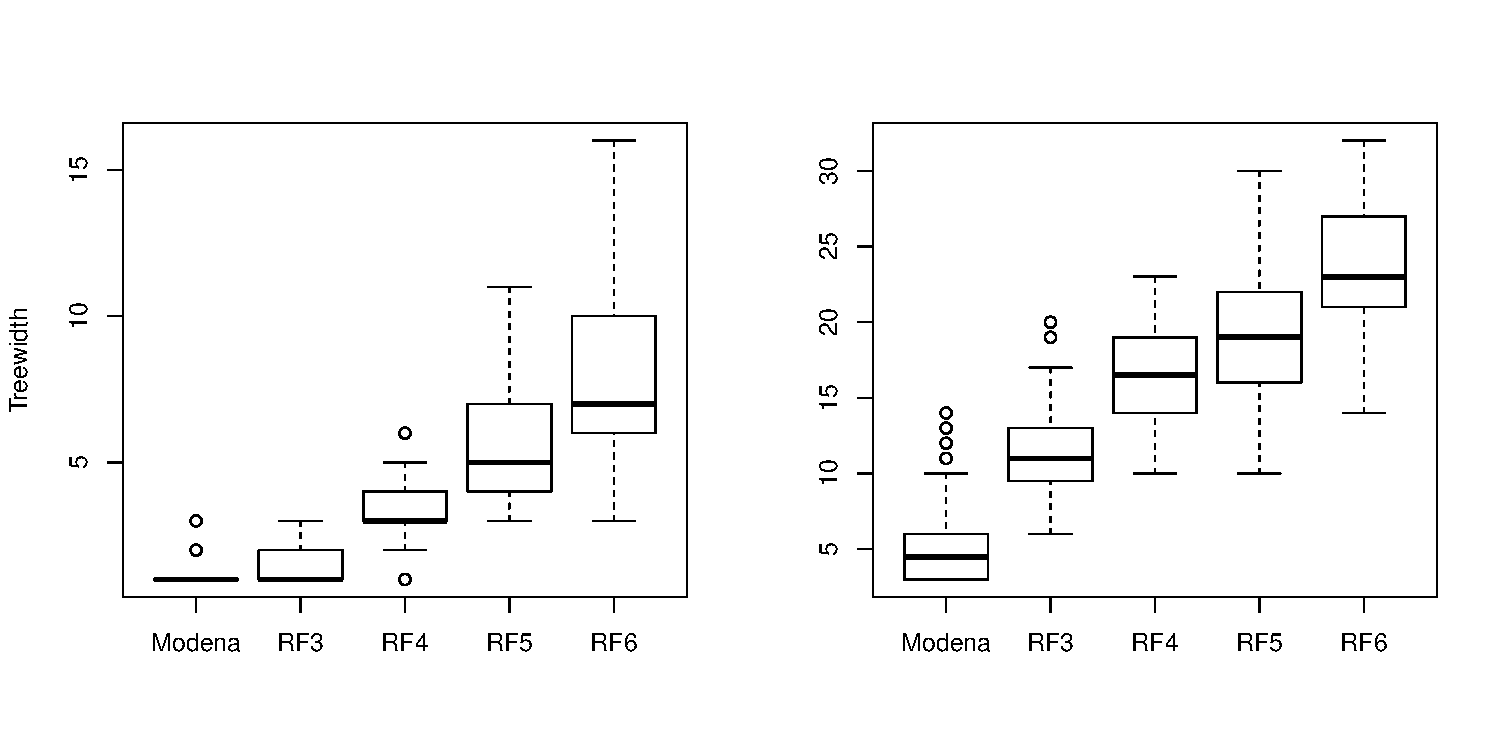
\includegraphics[width=\textwidth,trim=350 0 0 50,clip]{Figs/td-widths}
\end{minipage}
	  \begin{minipage}{.6\textwidth}\centering
	{\sffamily {\bfseries B} -- Correlation plot}\\
	  	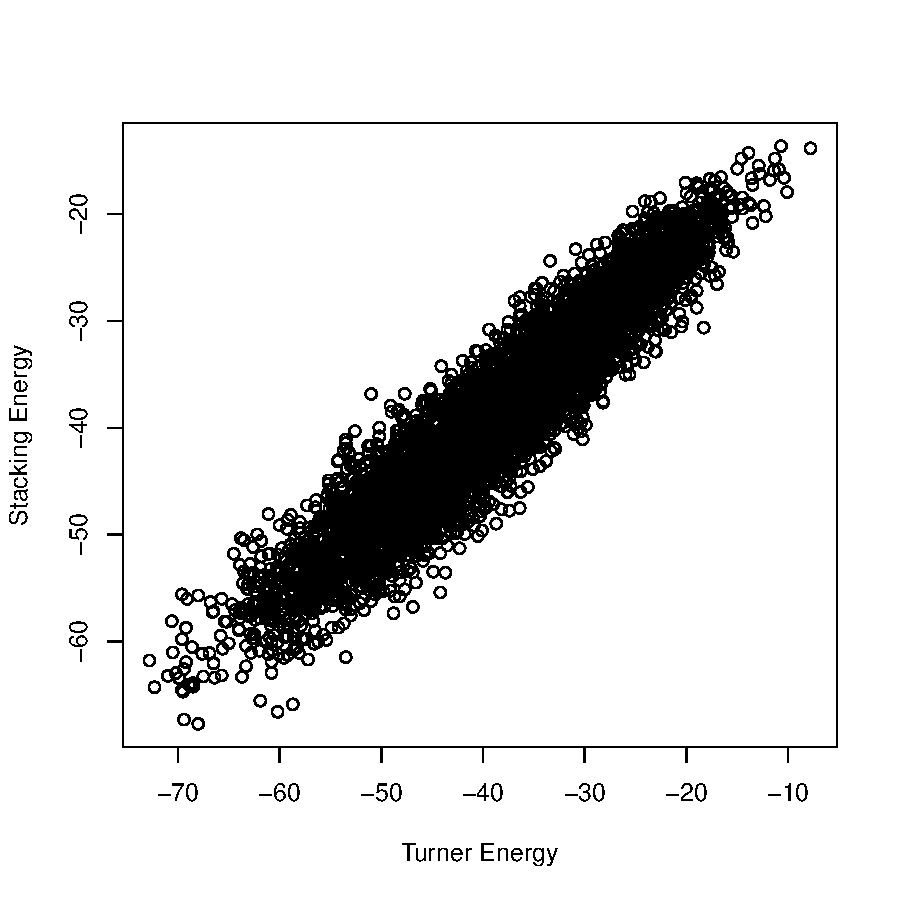
\includegraphics[width=\textwidth,trim=0 0 0 50,clip]{Figs/stackingcor} 
  	\end{minipage}
	  
        \caption{\revisedOne{A fitted energy model based on stacking pairs ({\sffamily\bfseries A}) leads to approximated free-energies that are highly correlated (R=0.99) with free-energies in the Turner energy model ({\sffamily\bfseries B}), yet induces tree widths that are amenable to practical sampling ({\sffamily\bfseries C})}.}
      \label{fig:correlation}
\end{figure}

\revisedOne{%
However, while in principle feasible, sampling in a Boltzmann distribution directly using the Turner energy model may induce extreme computational demands, with treewidths scaling at least as large as the number of nucleotides in the largest loop. Fortunately, we found that intricacy of the Turner energy model can be circumvented with minimal loss of precision by using a simpler stacking energy model. As shown in Figure~\ref{fig:correlation}, a simple stacking energy model, whose design principles are further described in Additional file~1: Section~\ref{appsec:modelparameters}, can be used to approximate the Turner energy model very adequately (correlation coefficient $R=0.99$) in the context of sequence design. Using this simpler model greatly reduces the treewidth, and thus the computational requirements of the whole method even for complex instances.
}

\subsection*{Effectively targeting Turner energies using multi-dimensional sampling}
\revisedOne{
We used our Boltzmann sampling strategy (Algorithms
\ref{alg:pf} and \ref{alg:sampling}), to sample valid sequences for
given target structures and weights $\pi_1,\dots,\pi_k$.  Moreover, we
used multi-dimensional Boltzmann sampling to target specific energies and
\GCb\%.  Our tool \ourprog{} evaluates energies according to the
stacking energy model $\EnergyStacking$, whose parameters were fitted
to best approximate Turner energies. As well, we implemented and
fitted a base pair energy model for \ourprog{}, which was not studied
for its targeting performance (both models:
Additional file~1: Section~\ref{appsec:modelparameters}).
%
%\paragraph{Implementation of multi-dimensional Boltzmann sampling}
%As suggested in Section~\ref{sec:multiBoltzmann}, we heuristically optimize weights to target specific energies and \GCb\% in an iterative procedure (based on the core sampling algorithm).
%Specifically, energy weights are initialized as $w_\ell=e^{\frac{1}{RT}}$; the gc weight as $w_{gc}=1$. For each iteration, $\psi\cdot n$ sequences are sampled with the current weights. Then, we determine the mean energies $E(S;R_\ell)$ and the mean GC content over the sampled sequences. For the next iteration, the weights are updated by the rules $w_\ell = w_\ell \gamma^{mean(E(S;R_\ell))-E_\ell}$ and $w_{gc} = w_{gc}\frac{GC_{target}}{mean(GC)}$. During this procedure, we collect   in a set $P$ all the sequences exhibiting energies within $[E_1-\delta,E_1+\delta]\times [E_2-\delta,E_2+\delta]\ldots$ and GC-content within $[GC_{target}-\idelta',GC_{target}+\delta']$.
%If $|P| > n$ or a maximum amount of iterations is reached, the sequences in $P$ are returned.
%


Fig.~\ref{fig:energydist-pk} illustrates how well complex realistic energy models can be approximated based on simpler, but better tractable ones. For
the two target structures of Fig.~\ref{fig:energydist-pk}B,
Fig.~\ref{fig:energydist-pk}A shows the good fit between realistic
energies in the full-fledged Dirks and Pierce energy model for
pseudoknots (D\&P model) and energies in the stacking energy
model\revisedOne{, which is obtained for each of the two target structures (with respective $R^2$ values of $0.846$ and $0.841$)}. For the shown fits we sampled $n=10\,000$ sequences, targeting a
\GCb\% of $60\%$.
%
For an example instance of the \texttt{Modena} benchmark with two
pseudoknotted target structures, Fig.~\ref{fig:energydist-pk}B shows
the Turner energy distributions of the single structures as they
result from sampling with different weight parameters. The figure
illustrates how our multidimensional Boltzmann sampling strategy can,
to a large extent, independently shift the Turner energies of sampled
sequences towards prescribed targets. See Additional file~1: Section~\ref{appsec:illustrating-mdbs} for a further example with three
pseudoknot-free target structures.}


%To reduce the cost of the precomputation, we used a stacking energy model
%as a proxy for the Turner model. Indeed, we observed a strong linear
%dependency between the Turner energy and the
%emphasize that only the simple stacking energies are directly targeted
%(at $\pm$10\% tolerance, except for a few hard instances). Due to our
%linear adjustment, we finally achieve well-controlled energies in the
%realistic Turner energy model.
\begin{figure*}[t]
  \begin{center}
    %{\sf \bfseries A}\
    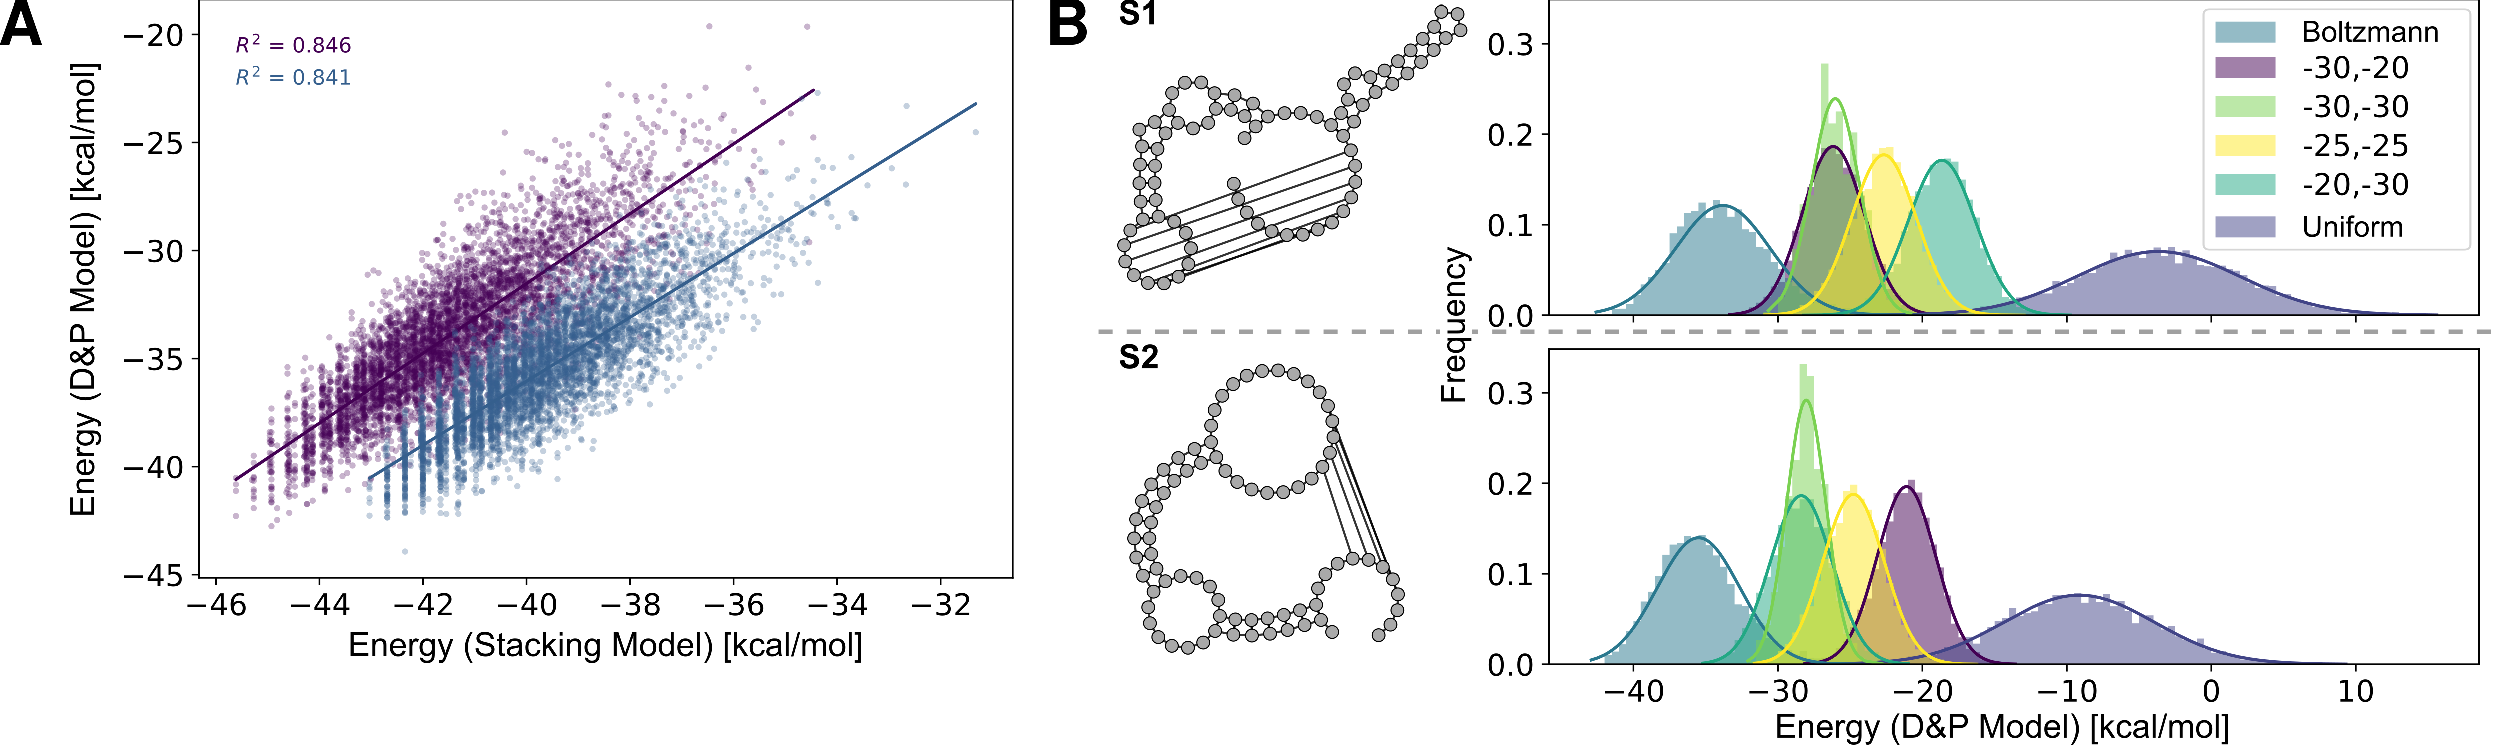
\includegraphics[width=0.97\textwidth]{Figs/energy_shift}\hfill
    %{\sf \bfseries B}\ \includegraphicstop[width=0.55\textwidth]{Figs/PKB00211_PKB00239_0_energy_distribution}
  \end{center}
  \caption{%
    Targeting specific energies for pseudoknotted structures using
    multi-dimensional Boltzmann sampling. \textbf{(A)} Linear fits between the
    energies in the stacking model to the realistic pseudoknot energy
    model by Dirks and Pierce (D\&P) for \revisedOne{initially} sampled sequences and both target structures R1 and R2 (shown in B). The good
    match \revisedOne{(respective $R^2$ values of $0.846$ and $0.841$)} enables more efficient targeting of Turner energies based on
    targeting stacking model energies. \textbf{(B)} \revisedOne{Resulting D\&P energy distributions for the two target structures R1 and R2 when aiming for the respective free energies $-30$ and $-20$,
    $-30$ and $-30$, $-25$ and $-25$, $-20$ and $-30$\,kcal/mol. These demonstrate the effectivity of our adaptive
    multi-dimensional Boltzmann sampling procedure, especially by} comparing the distributions to those of uniform and Boltzmann sampled sequences, with homogeneous weights $1$ and
    $e^\beta$, respectively.
%    ($\delta=0.05, \delta'=0.1, \gamma=1.1, \psi=20, n=1000$)
  }
  \label{fig:energydist-pk}
\end{figure*}

\subsection*{Generating high-quality seeds for further optimization}
We empirically evaluated \ourprog{} for generating seed sequences targeting multiple (pseudoknotted) structures, possibly followed by subsequent local optimizations. As a baseline for comparison, we considered \RNAblueprint~\citep{Hammer2017}, the current leading tool for multiple design.
As a quality measure, we applied the objective function introduced by~\citet{Hammer2017} \revisedOne{based on \cite{Flamm2001,HoenerzuSiederdissen2013}} for multi-stable design, defined as:
% \begin{align}
%   f(S)= \quad & \frac{1}{k} \sum_{\ell=1}^{k} (E(S, R_\ell) - G(S))\notag\\
%    & +\ \xi \frac{2}{k(k-1)} \sum\limits_{1\leq\ell<j\leq k}|E(S,R_\ell) - E(S,R_j)|.
% \end{align}
\begin{multline}
  \label{eq:blueprintobjective}
    \Obj(S) = \frac{1}{m} \sum_{\ell=1}^{m} (E(S, R_\ell) - \EnsE(S))\\
    +\frac{1}{2\binom{m}{2}} \sum\limits_{1\leq\ell<j\leq m}|E(S,R_\ell) - E(S,R_j)|,
\end{multline}
%
where the free energies $E(S, R)$ as well as the \Def{ensemble free energy} $\EnsE(S)$ of $S$ are computed
by {\tt RNAfold}~\citep{Lorenz2011} in the pseudoknot-free case; for
pseudoknotted targets, $\EnsE(S)$ is approximated by the \Def{minimum
  free energy} of $S$ as estimated by {\tt HotKnots}~\citep{Ren2005} in the energy model
of~\citet{dirks-pierce-03}.  Intuitively, the first term of \Obj{}
captures the distance of the targets from the ensemble free energy,
while the second term penalizes the dispersion of targets; \Obj{} is
best (minimized) when all targets simultaneously achieve the minimum
free energy of the sequence.

We considered a benchmark of six sets of target structures described in \citep{Taneda2015}: {\sf 2str}, {\sf 3str}, and {\sf 4str} consist of non-pseudoknotted structures, while {\sf PK60}, {\sf PK80}, and {\sf LE80} contain pseudoknotted structures.
%%For each instance of the \Software{Modena}
%benchmark~\citep{Taneda2015}, we generated $1\,000$ seed sequences at these energies.
%Our procedure is tailored to produce sequences with similar Turner
%energy that favor the stability of the target structures having
%moderate \GCb\%; all these properties are desirable objectives
%for RNA design.
\revisedOne{Based on} \ourprog{}, we generated at least 1\,000 seed sequences with similar energies for all target structures, for
each instance of the benchmark. 
For this purpose, we determine good common target energies that
can be successfully targeted for all single target structures simultaneously.
Generally, we targeted 60\% \GCb\%.
\revisedOne{%
Additional file~1: Section~\ref{appsec:effectivity-seed-generation} provides detailed results from this iterative procedure, which works similarly to the previously described multi-dimensional Boltzmann sampling. In particular, we observe that most of the benchmark inputs finish within only few iterations, where each iteration requires  little time (confer Additional file~1: Section~\ref{appsec:run-times}).}

We compared the
\Obj{} value of \revisedOne{the derived} sequences against that of seed sequences,
uniformly sampled using \RNAblueprint{}.  Moreover, for both sets we
used an adaptive greedy walk~\citep{Hammer2017} to \Def{minimize} the
\Obj{} function. At each step, the local search re-samples (uniformly
at random) the positions of a randomly selected component in the base
pair dependency graph, accepting the modification only if it results
in a gain. We performed 500 greedy descent steps in the case of
pseudoknot-free data-sets {\sf 2str}, {\sf 3str}, and {\sf 4str}; and
200 steps for the pseudoknotted ones {\sf PK60}, {\sf PK80}, and {\sf
  LE80}.


The results, shown in Fig.~\ref{fig:benchmark-results}, reveal that
Boltzmann-sampled sequences outperform uniform seeds on every data-set,
leading to average improvements in \Obj{} values ranging from $7.26$
({\sf LE80}) to $16.05$ ({\sf 2str}) units. Remarkably, this
improvement is observed for both terms in \Obj{} (see
Additional file~1: Section~\ref{appsec:contributions-multidefect}).  This means that \ourprog{}
produces sequences whose targets are substantially closer to
the ensemble free energy \emph{and} have more similar stability across targets.  In fact, for
every sequence in our benchmark, consisting of 332 sets of target
structures, we observed better \Obj{} for Boltzmann sampling than for
uniform sampling (see Additional file~1: Section~\ref{appsec:detailed-benchmark-results}).  Notably,
\ourprog{} performs equally well in the presence of pseudoknots;
the difficulty rather lies in the computation of the \Obj{} function, since
free energy minimization is costly in the presence of
pseudoknots~\citep{Sheikh2012} and good implementations are scarce.

%
Moreover, for all instances as well, the Boltzmann designs
remain superior even after local optimizations, as shown by
todo~\ref{fig:benchmark-results} and Additional file~1: Section~\ref{appsec:contributions-multidefect}
and \ref{appsec:detailed-benchmark-results}. This observation is consistent with a
superior quality of the starting point for the greedy walk, probably leading
to better local minima of the \Obj{} function. However, it should be noted
that the greedy walk is based on the uniform sampling of
\RNAblueprint{}, and thus can be expected to partially level the
advantages of Boltzmann sampling. In future work, we hope to improve
this aspect by exploiting Boltzmann sampling during the
optimization run.

%\begin{table}[t]
%\centering
%\medskip
%\begin{tabular}{@{}>{\bf}l@{\quad}>{\tt}l@{\quad}@{\quad}c@{\quad}c@{\quad}c@{}}
%  &   \textbf{\textrm{Dataset}}   & {\bfseries\ourprog{}} & \textbf{\RNAblueprint} & \textbf{$\Delta$-Improvement}\\ \toprule
%  Seeds      & 2str & 21.69 ($\pm$4.37) & 37.74 ($\pm$6.45) & 16.05\\
%             & 3str & 18.10 ($\pm$3.98) & 30.49 ($\pm$5.41) & 12.39\\
%             & 4str & 20.15 ($\pm$3.83) & 32.32 ($\pm$5.23) & 12.17\\
%             \cline{2-5}
%             & PK60 & 12.12 ($\pm$3.04) & 19.81 ($\pm$4.24) & 7.69\\
%             & PK80 & 13.81 ($\pm$3.63) & 24.05 ($\pm$4.93) & 10.24\\
%             & LE80 & 10.54 ($\pm$2.77) & 17.80 ($\pm$4.17) & 7.26\\
%             \midrule
%
%  Optimized  & 2str & 5.42 ($\pm$1.27) & 7.95 ($\pm$1.75) & 2.52\\
%             & 3str & 5.10 ($\pm$1.10) & 7.04 ($\pm$1.52) & 1.94\\
%             & 4str & 9.17($\pm$1.51) & 13.25 ($\pm$2.13) & 4.17\\
%             \cline{2-5}
%             & PK60  & 3.84 ($\pm$1.22) & 6.45 ($\pm$1.84) & 2.60\\
%             & PK80* & 3.41 ($\pm$1.59) & 7.99 ($\pm$2.35) & 4.42\\
%             & LE80  & 3.59 ($\pm$1.11) & 5.88 ($\pm$1.59) & 2.28\\
%             \bottomrule
%\end{tabular}\\[1em]
%
%\caption{Comparison of the multi-stable design objective function
%  (Eq.~(\ref{eq:blueprintobjective}) of sequences sampled by
%  \ourprog{} vs.\ uniform samples for three benchmark sets; before
%  (seeds) and after optimization (optimized). We report the average
%  scores with standard deviations; smaller scores are better. The
%  final column reports our improvements due to Boltzmann sampling over
%  uniform sampling (as difference of mean scores).}
%\label{tab:benchmark-results}
%\end{table}


\begin{figure}
  {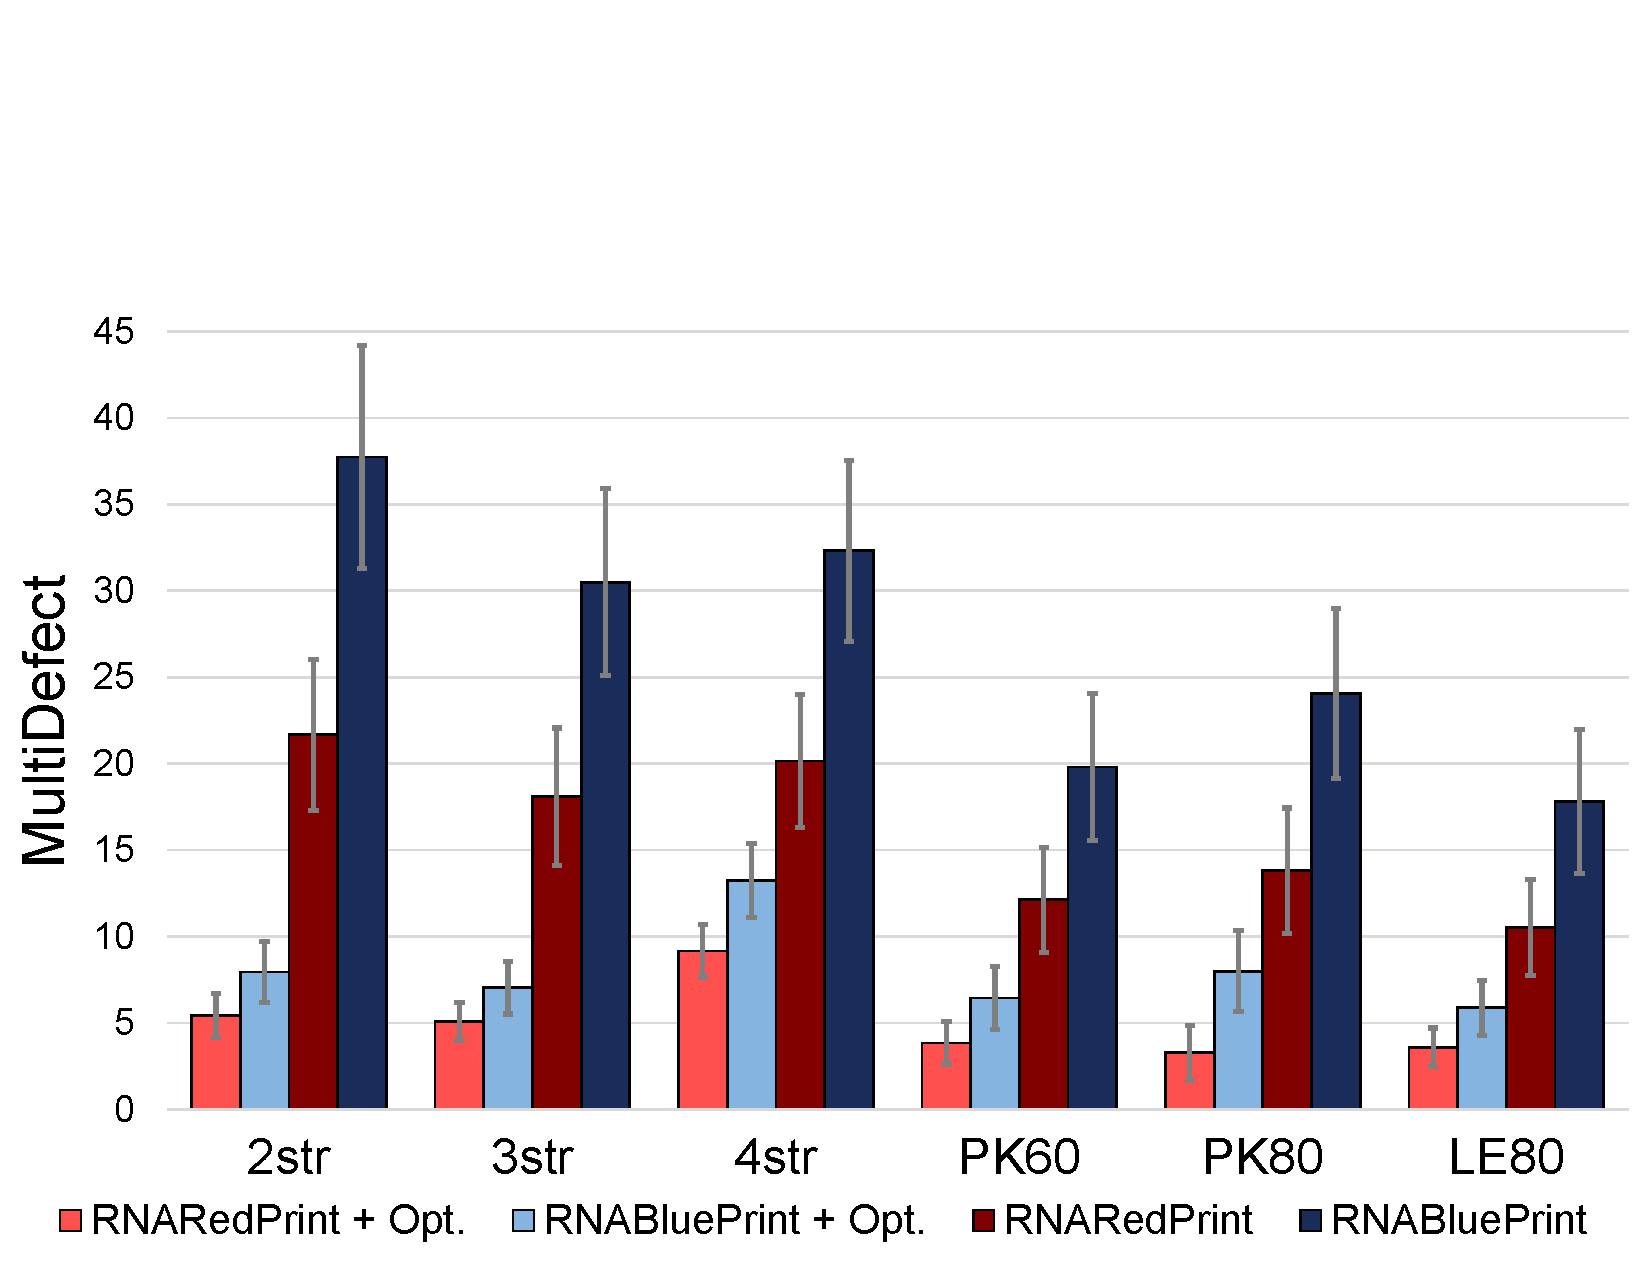
\includegraphics[width=.9\linewidth,trim={.2cm .3cm .2cm 5cm},clip]{Figs/statistics-overall}}
  \caption{Comparison of the \Obj{} (see
    Eq.~\eqref{eq:blueprintobjective}; smaller values $\to$ better
    designs) for sequences sampled by \ourprog{} and uniform sampling
    (\RNAblueprint) for six benchmark sets. For both sampling schemes,
    we show the MultiDefects of the sampled sequences, as well as
    results after further optimization by local search (``+ Opt.'').}
\label{fig:benchmark-results}
\end{figure}

\section*{Conclusion}
%%!!!!!!!!!!!!!!! consider to merge into discussion
%Going beyond our encoding of the base pair model energy features and the \GCb\% feature, the contributions provide more generality and allow expressing complex features of the
%sequences alone, e.g.\ rewarding or penalizing specific sequence
%motifs, as well as features depending on the target structures.
%Furthermore, constraints, which enforce or forbid features, are
%naturally expressed by assigning infinite penalties to invalid
%(partial) sequences (even if in implementations, explicit handling of constraints is advantageous). In particular, the %framework
%captures various RNA energy models, they can be handled efficiently (in the sense of FPT), as long as the dependencies of their additive energy contributions are bounded.

\revisedOne{Based on a general framework and efficient algorithms, we introduce a novel approach to design RNA
sequences while targeting very specific complex properties}. In particular, we describe the targeting of the free energies of multiple target structures and the \GCb-content.
%
Our method combines a fixed-parameter tractable (FPT) sampling algorithm
with multi-dimensional Boltzmann sampling over distributions
controlled by expressive RNA energy models. \revisedOne{We demonstrate that the approach, despite of its theoretical hardness, performs well on typical multi-stable RNA design instances in practice. This good performance is a direct consequence of the approximability of Turner energies as well as the systematic algorithmic framework. By conducting a proof-of-concept study 
  on an established benchmark set for negative multi-target RNA design (including pseudoknotted instances), we showcase a typical application of our tool \ourprog{}. In this study, 
  the approach generates significantly better seed sequences than
the previously best available method (uniform sampling). Our results strongly suggest that the presented technique for positive design can be highly beneficial in future negative design approaches.
}%
%
% SW--we have written most of this already:
%In this way, we as well demonstrated the practical feasibility of such controlled %sequence generation, including the case of pseudoknotted structures.
% YP--Stick to the present tense if you write anything new :) (or move everything to past) 
%
%
To substantiate our work additionally, we establish the $\#${\sf P}-hardness of uniform sampling which,
from a complexity-theoretic point of view, motivates the FPT, tree decomposition-based nature of our method.  


\revisedOne{In this way, our framework enables new possibilities
in the field of RNA sequence design.}
%allowing to enforce additional
%constraints, like \GCb\%, while controlling the energy of
%multiple target structures.
%Thus, it presents a major advance over
%previously applied ad-hoc sampling and even efficient %uniform sampling
%strategies. 
%
%perspectives:
\revisedOne{As particular advantage over previous sequence generation methods,} it is extensible to include various more complex sequence constraints, including mandatory/forbidden motifs at specific
positions or anywhere in the designed sequences, by adapting formal language constructs
of Zhou \emph{et al}~\citet{Zhou2013}. In future work, negative design principles could 
be explicitly supported at the generation stage, for instance by
penalizing a set of alternative helices/structures.
%
\revisedOne{We moreover envision using positive design to assess the significance of observed properties. Critically, our current perception of statistical significance suffers from overly simplistic simple null models (\emph{e.g.} dinucleotide shuffling) used to model random RNAs~\cite{Rivas2017}). Here, our approach promises fundamental improvements by constructing null models of random sequences that satisfy multiple complex constraints.} 




%%%%%%%%%%%%%%%%%%%%%%%%%%%%%%%%%%%%%%%%%%%%%%
%%                                          %%
%% Backmatter begins here                   %%
%%                                          %%
%%%%%%%%%%%%%%%%%%%%%%%%%%%%%%%%%%%%%%%%%%%%%%

\section*{Additional file}

\subsection*{Additional file 1}
\revised{The Supplemental Material contains additional
information on methods and parameters; elaboration of theory and proofs; and additional and detailed empirical results.}
% 
% \revised{Supplemental Material providing additional detailed information on 
% ``Immediate benefits of positive design for negative design'', ``Tree decomposition for RNA design instances in
% practice'', ``Run times for Boltzmann sampling (at fixed weights)'', ``Illustrating multi-dimensional Boltzmann sampling
% for three pseudoknot-free target structures'', ``Effectivity of the seed sequence generation'', ``Parameters for the
% base pair and the stacking energy model'', ``Tree decomposition with hyper-dependencies'', ``Correctness of the FPT
% partition function algorithm'', ``General complexity of the partition function computation by cluster tree elimination
% and generation of samples'', ``Exploiting constraint consistency to reduce the complexity'', ``Monotonicity of the
% partial derivatives within weight calibration'', ``Approximate counting and random generation'', ``Contribution of terms
% to the MultiDefect score'', and ``Detailed results of the negative design benchmark''.}

\begin{backmatter}
%%%%%%%%%%%%%%%%%%%%%%%%%%%%%%%%%%%
%%                               %%
%% Additional Files              %%
%%                               %%
%%%%%%%%%%%%%%%%%%%%%%%%%%%%%%%%%%%

\section*{Abbreviations}
\GCb\%: GC-content; \#P: complexity class ``Sharp P''; DP: dynamic programming; FPT: fixed-parameter tractable; D\&P
model: pseudoknot energy model by Dirks and Pierce

\section*{Availability of data and materials}
The software and data of this work are maintained in the Github repository
\url{https://github.com/yannponty/RNARedPrint}\revised{; the acrchived version referenced in this manuscript is
available at \href{https://dx.doi.org/10.5281/zenodo.2597571}{doi:10.5281/zenodo.2597571}.}

\section*{Author's contributions}
  YP and SW initiated the project and designed the algorithms.
  % SW---I guess we don't need to be super-detailed, otherwise something like...
  %YP contributed the multi-dimensional Boltzmann sampling background and the \#P-hardness proof.
  %SW contributed the integration with the constraint network setting and its specialization to RNA design.
  YP, SW and WW wrote the core software, while SW and SH contributed the weight optimization scripts. SH, SW and YP devised the computational experiments, which were conducted by SH. All authors wrote, read, and approved the manuscript.
    % Text for this section \ldots
    % https://www.biomedcentral.com/getpublished/editorial-policies#authorship

\section*{Funding}
YP is supported
%jointly supported
by the
% French
{\em Agence
  Nationale de la Recherche} and the
%Austrian
Austrian Science Fund (ANR-14-CE34-0011 and FWF-I-1804-N28; project RNALands).  SH is supported by the
German Federal Ministry of Education and Research (BMBF support code
031A538B; de.NBI: German Network for Bioinformatics Infrastructure)
and the
% acknowledged by
%financial support of the
Future and Emerging Technologies programme
% within the Seventh Framework Programme for Research of the
%European Commission, under
(FET-Open grant 323987; project RiboNets).
\revised{The funding bodies did not played any roles in the design
of the study and collection, analysis, and interpretation of data and in writing
the manuscript.}

\section*{Acknowledgements}
%
We thank Leonid Chindelevitch for suggesting a drastic optimization of our FPT algorithm based on stable sets combinatorics, and Arie Koster for practical recommendations on tree decompositions.
\revised{A preliminary version of this work was presented at the conference RECOMB 2019 in Paris; we acknowledge the
contributions of the anonymous reviewers.}

\section*{Ethics approval and consent to participate}
Not applicable.

\section*{Consent to publish}
Not applicable.

\section*{Competing interests}
  The authors declare that they have no competing interests.


%%%%%%%%%%%%%%%%%%%%%%%%%%%%%%%%%%%%%%%%%%%%%%%%%%%%%%%%%%%%%
%%                  The Bibliography                       %%
%%                                                         %%
%%  Bmc_mathpys.bst  will be used to                       %%
%%  create a .BBL file for submission.                     %%
%%  After submission of the .TEX file,                     %%
%%  you will be prompted to submit your .BBL file.         %%
%%                                                         %%
%%                                                         %%
%%  Note that the displayed Bibliography will not          %%
%%  necessarily be rendered by Latex exactly as specified  %%
%%  in the online Instructions for Authors.                %%
%%                                                         %%
%%%%%%%%%%%%%%%%%%%%%%%%%%%%%%%%%%%%%%%%%%%%%%%%%%%%%%%%%%%%%

% if your bibliography is in bibtex format, use those commands:
\bibliographystyle{bmc-mathphys} % Style BST file (bmc-mathphys, vancouver, spbasic).
\bibliography{biblio}      % Bibliography file (usually '*.bib' )
% for author-year bibliography (bmc-mathphys or spbasic)
% a) write to bib file (bmc-mathphys only)
% @settings{label, options="nameyear"}
% b) uncomment next line
%\nocite{label}

% or include bibliography directly:
% \begin{thebibliography}
% \bibitem{b1}
% \end{thebibliography}

%%%%%%%%%%%%%%%%%%%%%%%%%%%%%%%%%%%
%%                               %%
%% Figures                       %%
%%                               %%
%% NB: this is for captions and  %%
%% Titles. All graphics must be  %%
%% submitted separately and NOT  %%
%% included in the Tex document  %%
%%                               %%
%%%%%%%%%%%%%%%%%%%%%%%%%%%%%%%%%%%

%%
%% Do not use \listoffigures as most will included as separate files

%\section*{Figures}
%   \begin{figure}[h!]
%   \caption{\csentence{Sample figure title.}
%       A short description of the figure content
%       should go here.}
%       \end{figure}
% 
% \begin{figure}[h!]
%   \caption{\csentence{Sample figure title.}
%       Figure legend text.}
%       \end{figure}

%%%%%%%%%%%%%%%%%%%%%%%%%%%%%%%%%%%
%%                               %%
%% Tables                        %%
%%                               %%
%%%%%%%%%%%%%%%%%%%%%%%%%%%%%%%%%%%

%% Use of \listoftables is discouraged.
%%
% \section*{Tables}
% \begin{table}[h!]
% \caption{Sample table title. This is where the description of the table should go.}
%       \begin{tabular}{cccc}
%         \hline
%            & B1  &B2   & B3\\ \hline
%         A1 & 0.1 & 0.2 & 0.3\\
%         A2 & ... & ..  & .\\
%         A3 & ..  & .   & .\\ \hline
%       \end{tabular}
% \end{table}

    
\end{backmatter}
\end{document}
